\documentclass[12pt, a4paper, oneside]{article}
\usepackage{../preamble}

\medskip

\title{Введение в базы данных}
\author{
\\
\\
Конспект основан на лекциях Корнеева Георгия Александровича\footnote{kgeorgiy.info}}
\date{}

\graphicspath{{assets/}}

\begin{document}
\maketitle
\tableofcontents
\pagebreak

\section{Теория}

\subsection{Развитие баз данных}
\subsubsection{Простые и структурированные файлы}

Простые файлы состоят из:
\begin{itemize}
	\item Заголовок -- название столбцов.
	\item Данные -- значения, разделённые запятой.
\end{itemize}
В структурированных файлах в заголовках написано не только название столбца, но и его тип и длина.

\begin{remark}
	В структурированной версии можно быстро искать запись по номеру, то есть прочитать заголовок и
	узнать сколько занимает одна запись,умножить на нужный номер и прочесть сразу нужную запись.
\end{remark}

Достоинства:
\begin{itemize}
	\item Простота чтения -- написать код который будет читать такие данные просто.
\end{itemize}

\begin{itemize}
	\item Сложность поиска -- не реализовать эффективный поиск которому не нужно было бы загружать всё в
	      память.
	\item Сложность обработки.
	\item Сложно хранить нетривиальные типы данных например даты - теряется информация на какой позиции
	      месяц, на какой день.
	\item Нет проверки целостности	(ограничений).
\end{itemize}

\subsubsection{Файловая система}

Устройство:
\begin{itemize}
	\item Файл -- одна запись.
	\item Иерархия записей -- иерарзия каталогов.
\end{itemize}

Достоинства:
\begin{itemize}
	\item Простота реализации.
	\item Структурированные данные.
\end{itemize}

Недостатки:
\begin{itemize}
	\item Сложно извлекать требуемые данные.
	\item Нет проверки целостности.
	\item Большое количество файлов.
\end{itemize}

\subsubsection{Иерархическая модель данных}

\begin{remark}
	Иерархия это хорошо, но использовать для этого файловую систему не эффективно.
\end{remark}

\paragraph{Деревья}
Отношение родитель -- ребёнок соответствует каталогу и его подкаталогам в файловой системе,  но не
будет выделяться по файлу для каждой записи, вместо этого записи с одинаковым типом будут
группироваться (благодаря этому не нужно будет лишний раз обходить файловую систему).

Достоинства:
\begin{itemize}
	\item Проверка целостности появляется благодаря стуктурированности (а именно связи родитель - ребёнок),
	      например можно проверять что у человека нет двух оценок по одному предмету (хотя в файловой системе
	      тоже можно было это делать).
	\item Последовательное расположение записей - ускорение выполнения запросов.
\end{itemize}

Недостатки:
\begin{itemize}
	\item Представление только древовидных структур.
	\item Нет отношения многие ко многим, например у множества студентов есть множество оценок по разным
	      предметам и родителем будет студен, а детьми оценки или наоборот, запросы к обоим этим множествам
	      выполниться эффективно не могут.
\end{itemize}

\subsubsection{Сетевая модель данных}

Обобщение иерархических баз данных, нет единой строгой иерархии, есть базовая иерархия и есть
дополнительные иерархии вида владелец -- запись

\enewline

Достоинства:
\begin{itemize}
	\item Представление всех типов связей (в том числе многие-ко-многим).
	\item Возможность описания структуры.
	\item Эффективность реализации -- эффективные запросы к обоим мн-вам из связи многие ко многим, но
	      эффетивность разная из-за последовательной записи, только записи базовой иерархии записаны
	      последовательно.
\end{itemize}

Недостатки:
\begin{itemize}
	\item Более сложная реализация.
	\item Жесткое ограничение структуры -- если мы не подумали о каком то виде запросов заранее, то возможно
	      для его исполнения придётся поднять все данные.
\end{itemize}

\subsubsection{Реляционная модель данных}
\paragraph{Хранение}

Данные хранятся в таблицах, также в таблицах хранится информация о связях, связи задаются в
запросах.

\enewline

Достоинства:
\begin{itemize}
	\item Представление всех типов связей-
	\item Гибкая структура данных -- можно задавать произвольные запросы.
	\item Математическая модель -- позволяет говорить что некоторые запросы эквивалентны, то есть запрос не
	      обязан исполняться как написан, мб исполнен любой эквивалентный запрос, выбирается самый
	      эффективный из эквивалентных и получается тот же самый результат что и при исходном запросе потому
	      что запрсы эквивалентны.
\end{itemize}

Недостатки:
\begin{itemize}
	\item Сложность реализации.
	\item Сложность представления иерархических данных.
	\item Сложность составления эффективных запросов.
\end{itemize}

\subsubsection{Объектные базы данных}
Цель -- хранить граф объектов, который уже находится в памяти, в базе данных. Обычная реализация --
слой трансляции в реляционную базу данных

\enewline

Достоинства:
\begin{itemize}
	\item Работа в терминах объектов а не записей.
	\item Логичное направление ссылок, например можем легко взять все оценки студента потому что есть
	      соответствующее отображение из студента в оценки.
\end{itemize}

Недостатки:
\begin{itemize}
	\item Сложность реализации.
	\item Сложность миграции схемы, например добавление поля объекту, в базе уже есть объекты без этого поля.
	\item Малая распространенность.
\end{itemize}

\subsubsection{NoSQL (Not only SQL)}

\paragraph{Основная мысль} Реляционные базы данных умеют слишком много -- они заточенны чтобы работать
одинаково эффективно в куче различных сценариев, а если у нас какой то один сценарий, то можно
оптимизировать ровно для него и написать эффективней.

\enewline

Различные типы:
\begin{itemize}
	\item Документ-ориентированне -- есть куча документов, важно что внутри них, главное уметь их быстро
	      искать.
	\item Ключ-значение -- всё что предоставляет движок - быстро по ключу достать значение.
	\item Табличные и столбчатые -- хранить таблицы по стобцам, так если у нас множество запросов к
	      конкретным двум столбцам, то мы сможем прочитать только их, читать придётся дважды (каждый столбец
	      отдельно читается), но зато не нужно читать все столбцы как в табличном подходе.
	\item Графовые -- хотим хранить графы.
\end{itemize}

Достоинства:
\begin{itemize}
	\item Большой выбор -- отказываемся почти от всего кроме одного, у чего получаем большую
	      производительность.
	\item Гибкость -- в момент разработки базы, не тогда когда уже есть база.
	\item Скорость работы.
\end{itemize}

Недостатки:
\begin{itemize}
	\item Множество вещей делается в коде.
	\item Нет стандартных оптимизаторов.
	\item Легко ошибиться.
\end{itemize}

\subsection{Архитектура РСУБД}

Есть программа, есть данные, и программа обращается к данным.

\paragraph{Протокол} Для взаимодействия нужен протокол, его реализуют драйвера, которые находятся
и на стороне программы, и на стороне СУБД, которая уже будет обращаться в хранилище. Могут быть
различные протоколы, традиционно у каждого субд есть свой протокол, по которому можно с ней
общаться

\begin{remark}
	СУБД и хранилище находятся на одном компьютере, благодаря этому нет передачи данных по сети во
	время исполнения запроса (если хранилище представляет из себя несколько компьютеров то
	взаимодействие по сети всё же есть).
\end{remark}

\paragraph{Запрос}
\begin{enumerate}
	\item Стандартный SQL запрос требуется разобрать, для этого есть модуль \textit{Разборщик запроса}, который
	      представляет из себя парсер.
	\item \textit{Исполнитель запроса} исполняет запрос, но так как исполнять ровно тот запрос
	      который написан не эффективно существует \textit{Оптимизатор}.
	\item \textit{Посторитель плана исполнения} или \textit{Оптимизатор} берёт разобранный
	      запрос и решает как он будет исполняться: какие, откуда и в каком порядке будут загружаться данные,
	      какие индексы будут использованы.
	\item Управление памятью - это важно для исполнителя, потому что от того поместятся все данные в память
	      или нет зависит эффективная реализация запроса.
	\item Статистика. Например нам нужно прочитать данные о всех студентах конкретного пола, либо мальчиков,
	      либо девочек, тогда имея статистику и том что их кол-во отличается на порядок оптимизатор может
	      понять что всех мальчиков будет быстрее прочитать просто читая все данные подряд, а девочек,
	      возможно при наличии способа быстро идентифицировать именно девушек, читая данные только о них.
\end{enumerate}

\begin{figure}[H]
	\centering
	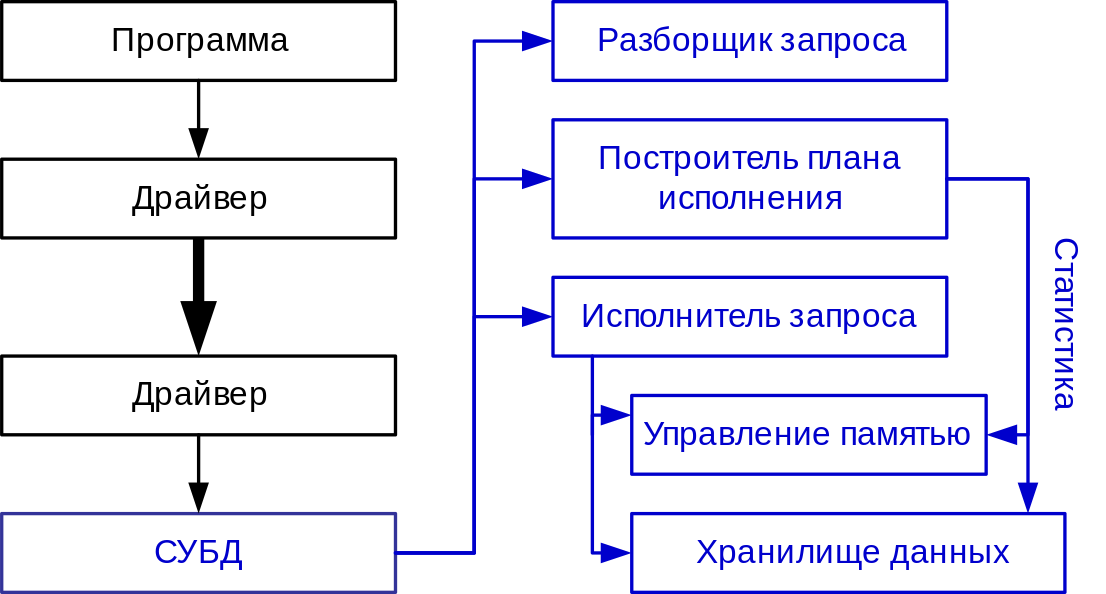
\includegraphics[width=0.8\textwidth]{../assets/kgeorgiy/intro/intro_arch_complete.svg.png}
	\caption{Полноценная схема}
	\label{rsubd-scheme}
\end{figure}

\subsection{Современные РСУБД}
\subsubsection{Корпоративные}

\paragraph{Корпоративные СУБД} - предназначены для продажи большим корпорациям, но у большинства
таких РСУБД есть девелоперские лицензии, которые позволяют использовать их в ограниченной среде (ограничение на кол-во ядер и размер памяти).

\begin{itemize}
	\item Oracle (Oracle)
	      \begin{itemize}
		      \item высокая пропускная способность (throughput)
		      \item невысокая скорость обновления (latency)
	      \end{itemize}
	      \begin{remark}
		      Два утверждения выше не противоречат друг другу, хотя каждый запрос и исполняется медленно, пропускная способность получается большой за счёт того, что конкретная СУБД заточена на исполнение тысяч параллельных запросов, и суммарная пропускная способность всех этих запросов, а не отдельных запросов, будет высокой.
	      \end{remark}
	\item DB2 (IBM)
	      \begin{itemize}
		      \item ориентация на «большие» машины, то есть с точки зрения IBM, СУБД это не приложение, которое крутится на сервере, а отдельное железо
		      \item мало распространена в России, так как развивалась в 60'е - 80'е годы предыдущего века
		      \item неполная совместимость с SQL
	      \end{itemize}
	\item SQL Server (Microsoft)
	      \begin{itemize}
		      \item работа под Windows
		      \item масштабируемость (путём добавления новых процессоров)
	      \end{itemize}
\end{itemize}

\subsubsection{Свободные}
\begin{itemize}
	\item MySQL
	      \begin{itemize}
		      \item поддерживаются различные форматы хранения БД
		      \item неполная поддержка SQL
		      \item есть enterprise и community версии
	      \end{itemize}
	\item PostgreSQL
	      \begin{itemize}
		      \item непосредственная поддержка связей - СУБД достаточно стабильна, чтобы использовать в реальных проектах
		      \item объектные расширения - но в то же время эта СУБД - экспериментальный проект, в который добавляется куча различных возможностей, некоторые из которых не выходят из экспериментального статуса
	      \end{itemize}
	\item Firebird
	      \begin{itemize}
		      \item была очень популярна когда делалась \href{https://en.wikipedia.org/wiki/Borland}{Borland}'ом под Delphi
		      \item используется только в старых проектах, так как в БД, которые используют это СУБД, есть данные, которые нельзя потерять, а перенести их очень сложно
	      \end{itemize}
\end{itemize}

\subsubsection{Встраиваемые}
\begin{itemize}
	\item SQLite
	      \begin{itemize}
		      \item компактна, поэтому много используется на мобильных устройствах
		      \item in-memory mode - все данные должны поместиться в память
		      \item ограниченная реализация SQL-92
	      \end{itemize}
	\item Apache Derby
	      \begin{itemize}
		      \item in-memory mode - умеет быть полностью in-memory, а также умеет работать с данными которые в память не поместились
		      \item хорошо совместим с DB2, так как был проектом IBM'а, и из-за этого же не очень хорошо совместим со всеми остальными
		      \item pure Java - встраивается в любое java приложение
	      \end{itemize}
	\item HyperSQLDB
	      \begin{itemize}
		      \item pure Java
		      \item не поддерживает транзакции
		      \item in-memory mode
		      \item в основном используется для тестирования
	      \end{itemize}
	\item Access
	      \begin{itemize}
		      \item совмещение СУБД и RAD
		      \item встраиваемые приложения
	      \end{itemize}
	      \begin{remark}
		      In-memory базы данных хорошо подходят для тестирования, потому что каждый пользователь может легко поднять свой instance из-за того что база in-memory и это всё ещё SQL, и каждому из instance'ов не будут мешать тесты других пользователей, также нет проблем с тем что схема данных может быть старой.
	      \end{remark}
\end{itemize}
\subsection{Модель сущность-связь}
\subsubsection{Сущность}
У сущности есть имя и атрибуты, атрибут представляет из себя имя, домен и свойства.
\begin{itemize}
	\item домен - информация о тех данных которые хранятся в атрибуте,конкретный физический тип будет выбран позже
	\item свойства - обязательный/не обязательный, основной ключ (Pk)/дополнительный ключ (Kn)
\end{itemize}

\begin{figure}[h]
	\centering

	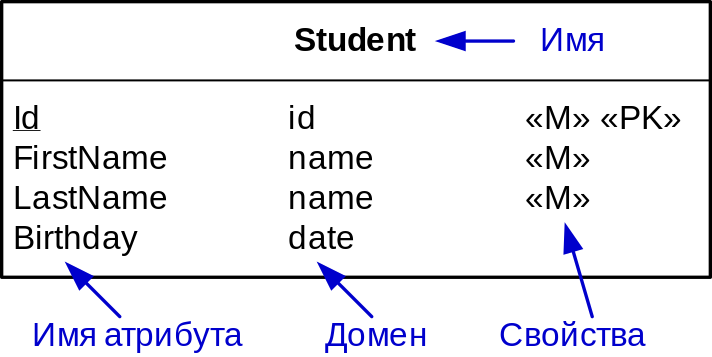
\includegraphics[width=0.8\textwidth]{../assets/kgeorgiy/modelling/ERModel_Entity.svg.png}
	\caption{Иллюстрация сущности}
\end{figure}

\subsubsection{Связь}
\paragraph{Связь} связывает несколько сущностей, имеет имя и тип. Тип связи обозначается на её
концах

% На рисунке \ref{end-types} приведены типы концов связей.

\begin{figure}[h]
	\centering

	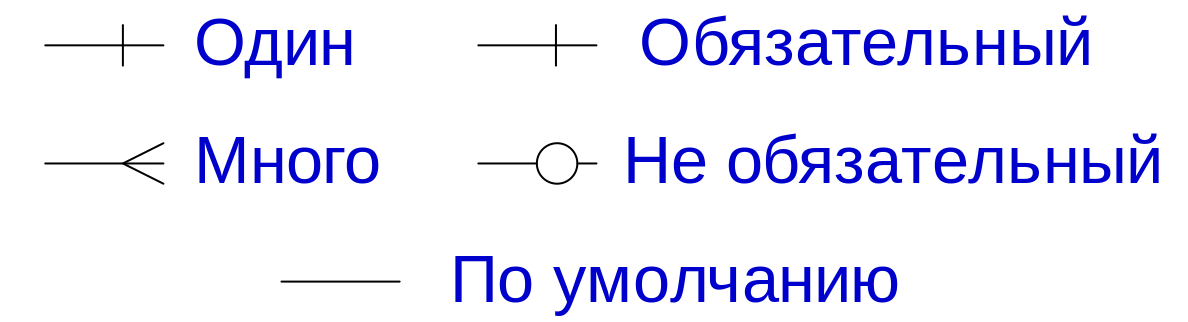
\includegraphics[width=0.8\textwidth]{../assets/kgeorgiy/modelling/ERModel_ArrowEnds.svg.png}
	\caption{Типы концов}
	%	\label{end-types}
\end{figure}

\begin{remark}
	Тут кривой рисунок, 'Один' - должна быть просто прямая линия, без значка обязательности
\end{remark}

%На рисунке \ref{ref-types} приведены типы связей.

\begin{figure}[h]
	\centering

	
\includegraphics[width=0.8\textwidth]{../assets/kgeorgiy/modelling/ERModel_RelationshipTypes.svg.pn
		g}
	\caption{Примеры связей}
	%	\label{ref-types}
\end{figure}

\subsubsection{Ассоциации}
\paragraph{Ассоциация} это некоторое обобщение связи, два типа обобщения:
\begin{enumerate}
	\item нагрузить связть, задать ей дополнительные свойства
	\item сделать многосторонней, больше чем два конца
\end{enumerate}

\begin{figure}[h]
	\centering

	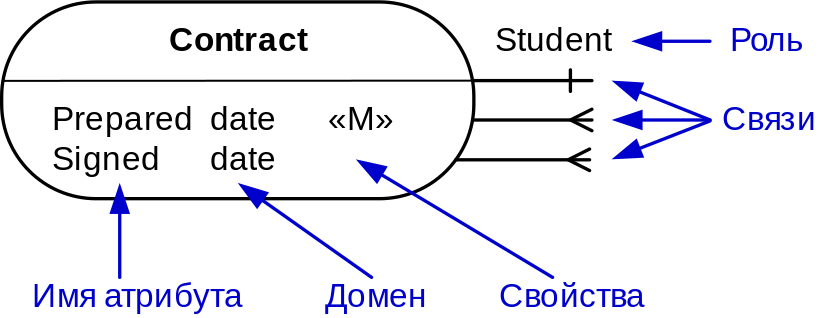
\includegraphics[width=0.8\textwidth]{../assets/kgeorgiy/modelling/ERModel_Association.svg.png}
	\caption{Пример ассоциации}
\end{figure}

\begin{remark}
	У ассоциаций, в отличии от обычных связей, есть название и атрибуты, но нет ключей, иначе они стали бы сущностями
\end{remark}

\begin{remark}
	Из-за того что у ассоциаций нет ключей, у них нет связей между собой
\end{remark}

\paragraph{Ограничения по Чену} (look-across, Chen-like), если зафиксировать все сущности кроме
одной, то получим ограничения на оставшуюся.

\paragraph{Ограничения по Мерис} (look-here Merise-like) - ограничение непосредственно на сущность

Обобщение ограничений:
\begin{figure}[h]
	\centering

	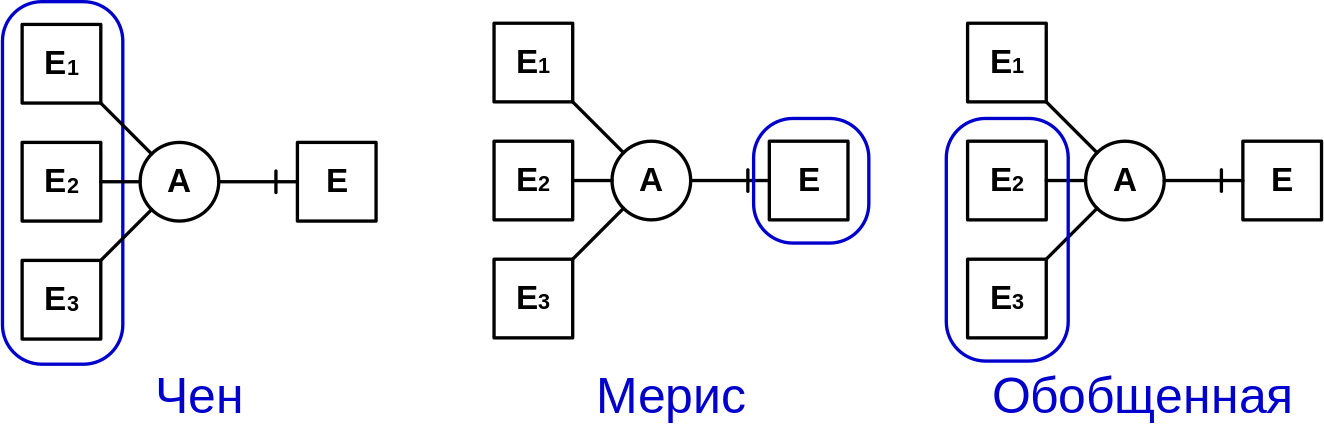
\includegraphics[width=0.8\textwidth]{../assets/kgeorgiy/modelling/ERModel_Multi_Generic.svg.png}
	\caption{Generic}
\end{figure}

\subsubsection{Слабая сущность}
Сущность, на которую можно сослаться, но у неё недостаточно атрибутов для её идентификации. Поэтому для слабой сущности вводится понятие идентифицирующей связи (которые рисуются двойной линией).

\subsection{Реляционная алгебра. Предназначение и свойства}
Базы данных нужно уметь не только проектировать, но и использовать. Существует
несколько способов формулировать запросы. Первый из рассматриваемых --
\textit{реляционная алгебра}.

\paragraph{Мотивация}
Действительно, в базах данных можно не только хранить данные, но и делать
выборки, изменять их каким-либо образом. Для этого вводится понятие запроса.
При первом рассмотрении, запросы нужны как минимум для выполнения следующих
действий:

\begin{itemize}
	\item Выборка данных: получить данные из базы, чтобы тем или иным способом
	      обрабатывать их уже извне.
	\item Область действия обновлений: запросы позволят указывать область действия тех
	      или иных операций, что крайне полезно. Например, к таким операциям относятся
	      операции удаления или изменения данных: хочется указывать, на какие именно
	      записи эти операции подействуют.
	\item Ограничения целостности: до сих пор было только два вида ограничений (ключи и
	      внешние ключи). Некоторые базы данных позволяют создавать произвольные
	      ограничения целостности, заданные на поддерживаемом языке. В рамках этих
	      ограничений очень удобно пользоваться запросами.
	\item Ограничения доступа.
\end{itemize}

\begin{definition}
	\textit{Реляционная алгебра} -- алгебра над множеством всех отношений.
	% TODO(dzhiblavi) добавить ссылку %
\end{definition}

Далее будут определены некоторые из операций (которые по определению должны
быть замкнуты над носителем), и ограничения, которые им соответствуют. В целом,
реляционная алгебра -- императивный язык для работы с отношениями, который
позволяет в явном виде, по действиям, описать, каким именно образом должен быть
получен результат.

\paragraph{Примеры} Рассмотрим несколько простых примеров операций в рамках
реляционной алгебры.
\begin{itemize}
	\item Проекция отношения на множество атрибутов: $\pi_{A}(R)$;
	\item Естественное соединение $R_1 \bowtie  R_2$.
\end{itemize}

\begin{remark}
	Как уже говорилось, все операции в рамках алгебры замкнуты по определению. Это
	означает, что их можно комбинировать произвольным образом (при сохранении
	условий на возможность исполнения операции). Например: $\pi_A(R_1
		\bowtie  \pi_B(R_2)) \bowtie  R_3$.
\end{remark}

\paragraph{Операции}
В текущем контексте полезно уточнить, что именно понимается под операцией над
отношениями в рамках реляционной алгебры. А именно, для того, чтобы определить
операцию, необходимо определить следующее:

\begin{itemize}
	\item Правило построения заголовка по заданным отношениям;
	\item Правило построения тела по заданным отношениям;
	\item Условия, при которых операция выполнима, то есть ограничения на отношения, к
	      которым она применяется.
\end{itemize}

\subsection{Реляционная алгебра. Унарные и множественные операции}

В этом разделе будут описаны унарные операции в рамках реляционной алгебры. В соответствии с
определением, для определения каждой операции нужно указать способ построения заголовка, тела
отношения, а также условия применимости, если такие есть.

\subsubsection{Проекция}

\begin{definition}
	\textit{Проекцией} отношения $R$ на множество атрибутов
	$A = \{ a_1, a_2, \ldots, a_n \}$ называется отношение, полученное из исходного путем
	удаления атрибутов не из $A$. Обозначается $\pi_A(R)$.
\end{definition}

Данная операция может быть полезна для следующего:
\begin{itemize}
	\item Привести отношение к виду, в котором над ним можно будет осуществить другую операцию (например,
	      объединение);
	\item Выбрать из отношения только нужные данные (для выборки).
\end{itemize}

На рисунке \ref{proj-def} приведена иллюстрация к определению $\pi_{A_2, A_4, A_5}(A)$.

\begin{figure}[h]
	\centering
	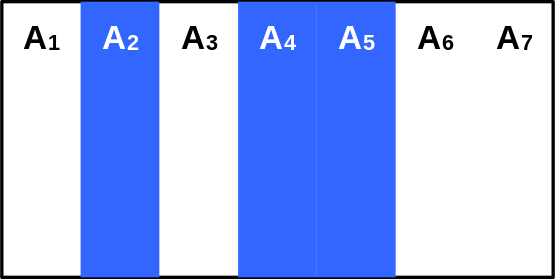
\includegraphics[width=0.8\textwidth]{../assets/kgeorgiy/relalgebra/Primitive_Projection_0.svg.png}
	\caption{Иллюстрация к определению проекции}
	\label{proj-def}
\end{figure}

Синим здесь обозначены столбцы, которые есть в результате операции. Остальные столбцы не
используются, и результат никак не зависит от их содержимого.

\paragraph{Примеры}
Приведем несколько тривиальных примеров применения проекции.

\begin{itemize}
	\item $\pi_{FirstName, LastName}$
	      \begin{figure}[H]
		      \centering
		      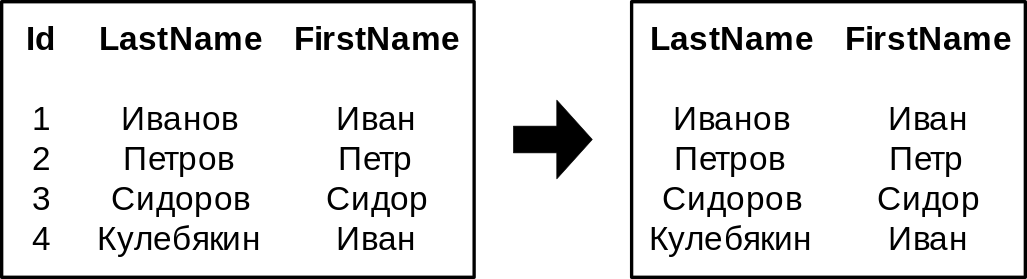
\includegraphics[width=0.8\textwidth]{../assets/kgeorgiy/relalgebra/Primitive_Projection_2.svg.png}
		      \caption{Проекция. Пример 1}
		      \label{proj-ex-1}
	      \end{figure}
	\item $\pi_{FirstName}$
	      \begin{figure}[H]
		      \centering
		      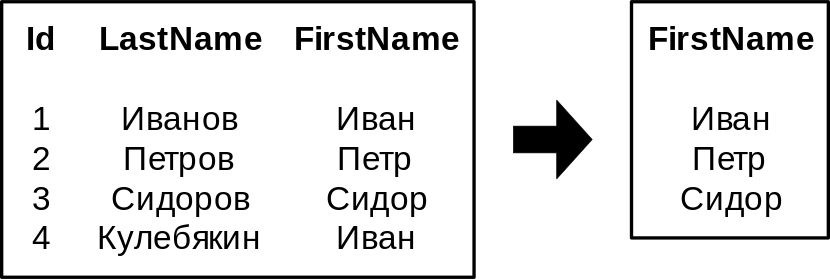
\includegraphics[width=0.8\textwidth]{../assets/kgeorgiy/relalgebra/Primitive_Projection_3.svg.png}
		      \caption{Проекция. Пример 2}
		      \label{proj-ex-2}
	      \end{figure}
\end{itemize}

\subsubsection{Фильтрация}

\begin{definition}
	\textit{Фильтрацией (селекцией, выборкой из)} отношения $R$ называется отношение,
	чей заголовок полностью совпадает с заголовком $R$, но тело содержит только
	кортежи, удовлетворяющее условию $c$. Обозначение: $\sigma_c(R)$.
\end{definition}

Операция часто используется для
\begin{itemize}
	\item Ограничения области действия изменяющих запросов;
	\item Получения выборки данных, соответствующих определенному условию.
\end{itemize}

На рисунке \ref{sel-def} приведена иллюстрация к определению $\sigma_c(R)$.

\begin{figure}[H]
	\centering
	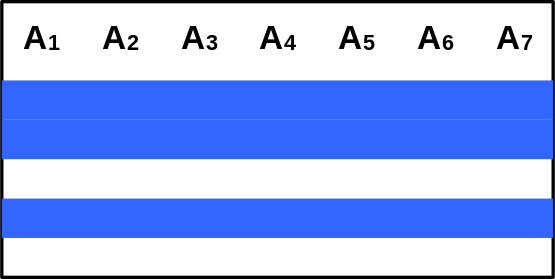
\includegraphics[width=0.8\textwidth]{../assets/kgeorgiy/relalgebra/Primitive_Section_0.svg.png}
	\caption{Иллюстрация к определению фильтрации}
	\label{sel-def}
\end{figure}

Синим здесь обозначены столбцы, которые есть в результате операции. Остальные столбцы не
используются, и результат никак не зависит от их содержимого.

\paragraph{Примеры}
Приведем несколько тривиальных примеров применения фильтрации.

\begin{itemize}
	\item $\sigma_{Id>2}$
	      \begin{figure}[H]
		      \centering
		      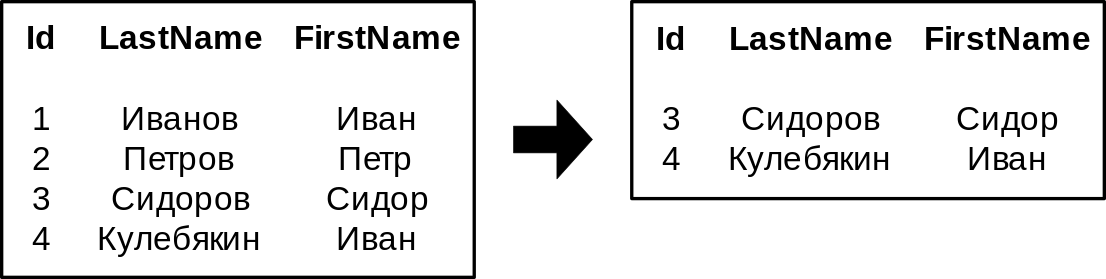
\includegraphics[width=0.8\textwidth]{../assets/kgeorgiy/relalgebra/Primitive_Section_2.svg.png}
		      \caption{Фильтрация. Пример 1}
		      \label{sel-ex-1}
	      \end{figure}
	\item Можно писать более сложные условия. $\sigma_{Id>2 \wedge FirstName=\texttt{Иван}}$
	      \begin{figure}[H]
		      \centering
		      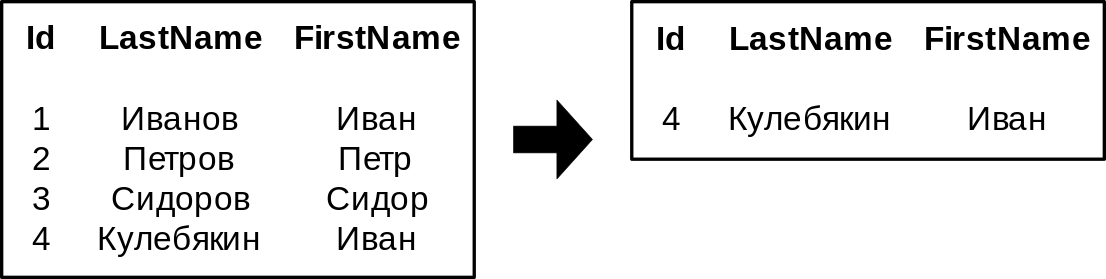
\includegraphics[width=0.8\textwidth]{../assets/kgeorgiy/relalgebra/Primitive_Section_3.svg.png}
		      \caption{Фильтрация. Пример 2}
		      \label{sel-ex-2}
	      \end{figure}
	\item Можно использовать функции, доступные в используемой БД. \\ $\sigma_{\texttt{length}(FirstName) + 2 \geqslant \texttt{length}(LastName)}$
	      \begin{figure}[H]
		      \centering
		      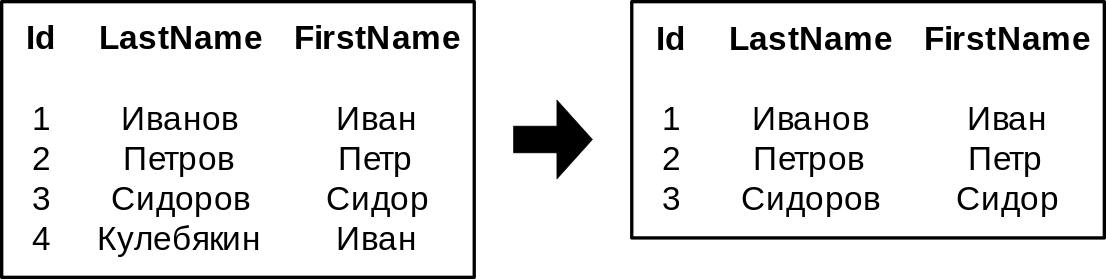
\includegraphics[width=0.8\textwidth]{../assets/kgeorgiy/relalgebra/Primitive_Section_4.svg.png}
		      \caption{Фильтрация. Пример 3}
		      \label{sel-ex-3}
	      \end{figure}
\end{itemize}

\subsubsection{Переименование}

\begin{definition}
	\textit{Переименованием} называется операция, при которой меняются названия
	атрибутов отношения. Тело при этом остается неизменным.
\end{definition}

Операция часто применяется для того, чтобы отношение можно было использовать в рамках другой
операции (например, при объединении с другим отношением).

\paragraph{Примеры}
Ниже приведен тривиальный пример-пояснение для операции переименования.

\begin{itemize}
	\item $\rho_{Name=FirstName, Surname=LastName}$
	      \begin{figure}[H]
		      \centering
		      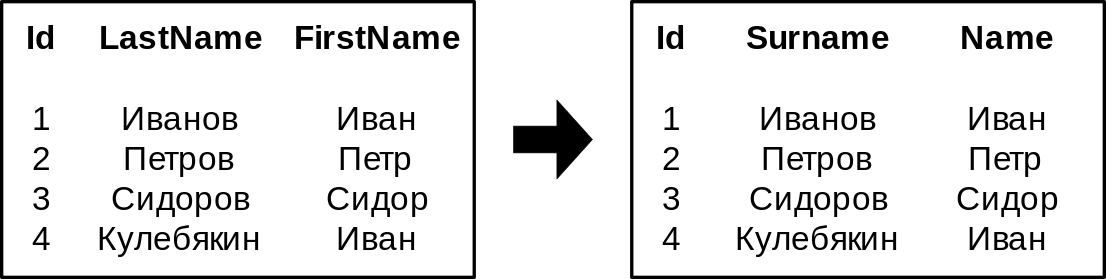
\includegraphics[width=0.8\textwidth]{../assets/kgeorgiy/relalgebra/Primitive_Rename_2.svg.png}
		      \caption{Переименование. Пример}
		      \label{ren-ex}
	      \end{figure}
\end{itemize}

\subsubsection{Множественные операции}

Из теории множеств в реляционную алгебру естественным образом переходят операции:
\begin{itemize}
	\item $R_1 \cup R_2$ -- объединение.
	\item $R_1 \cap R_2$ -- пересечение.
	\item $R_1 \setminus R_2$ -- разность.
\end{itemize}

Эти операции по определению применимы только к отношениям с одинаковыми заголовками. В результате
получается отношение с таким же заголовком и телом, полученным в соответствии с множественной
операцией. Иначе говоря, заголовок остается тем же, а над телами отношений производится
соответствущая множественная операция (объединение, пересечение, вычитание и прочие).

\paragraph{Примеры}
\begin{itemize}
	\item Объединение отношений: $R_1 \cup R_2$
	      \begin{figure}[H]
		      \centering
		      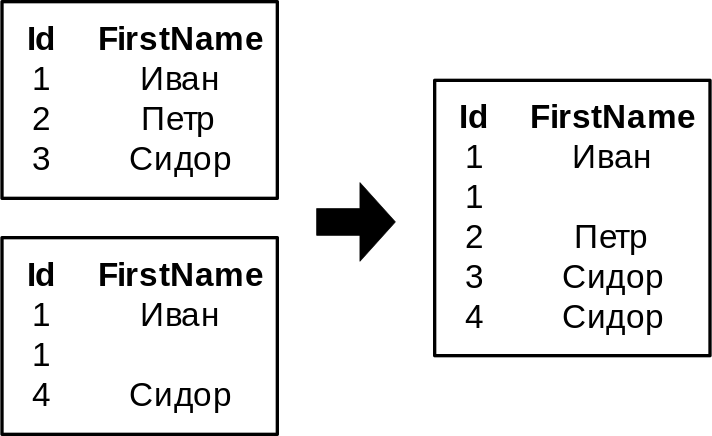
\includegraphics[width=0.8\textwidth]{../assets/kgeorgiy/relalgebra/Set_Union_2.svg.png}
		      \caption{Объединение отношений}
		      \label{set-union-ex}
	      \end{figure}
	\item Пересечение отношений: $R_1 \cap R_2$
	      \begin{figure}[H]
		      \centering
		      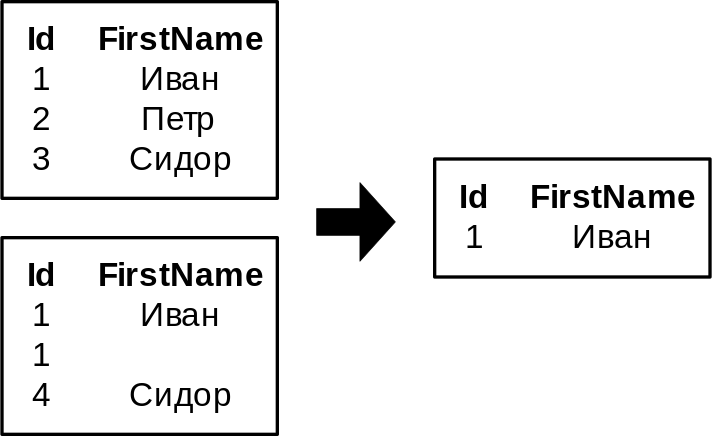
\includegraphics[width=0.8\textwidth]{../assets/kgeorgiy/relalgebra/Set_Intersect_2.svg.png}
		      \caption{Пересечение отношений}
		      \label{set-intersect-ex}
	      \end{figure}
	\item Разность отношений: $R_1 \setminus R_2$
	      \begin{figure}[H]
		      \centering
		      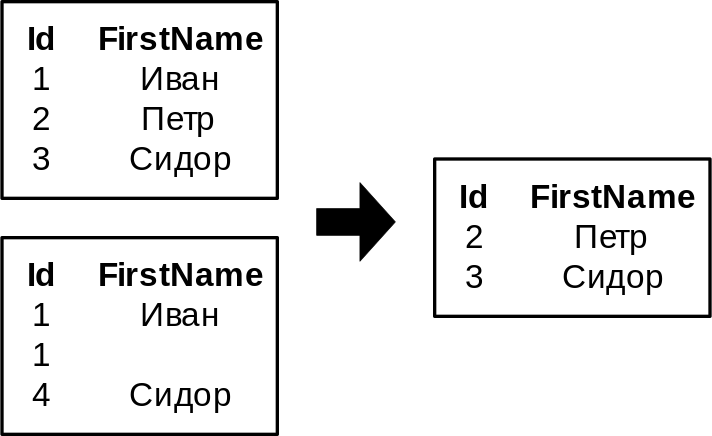
\includegraphics[width=0.8\textwidth]{../assets/kgeorgiy/relalgebra/Set_Minus_2.svg.png}
		      \caption{Разность отношений}
		      \label{set-minus-ex}
	      \end{figure}
\end{itemize}

Стоит отметить, что для объединения отношений с различающимися именами атрибутов, но при равном их
количестве, можно воспользоваться переименованием для того, чтобы привести заголовки к одному виду.

\subsection{Реляционная алгебра. Соединения}

\subsubsection{Полное соединение}

\begin{definition}
	\textit{Полным соединением} называется декартово произведение двух отношений. Заголовком
	является объединение заголовков, а телом -- декартово произведение тел отношений.
\end{definition}

\begin{remark}
	Необходимым условием выполнимости этой операции является отсутствие общих имен атрибутов. При
	желании, этого можно добиться операцией переименования (см. \ref{def-rename}).
\end{remark}

На рисунке \ref{full-join-ex} приведен пример полного соединения.

\begin{figure}[H]
	\centering
	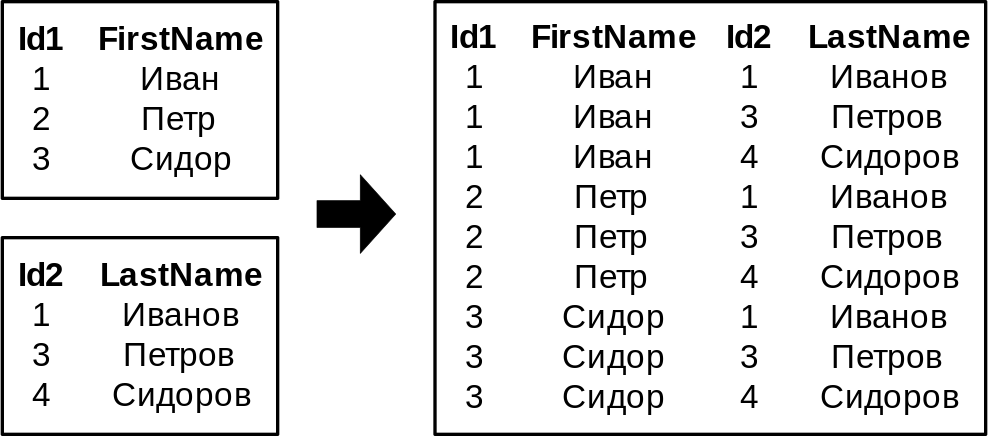
\includegraphics[width=0.8\textwidth]{../assets/kgeorgiy/relalgebra/Join_Full_2.svg.png}
	\caption{Пример полного соединения}
	\label{full-join-ex}
\end{figure}

\subsubsection{Естественное соединение}\label{nat-join-def}

\begin{definition}
	\textit{Естественным соединением} называется операция, при которой у двух отношений соединяются
	кортежи, имеющие равные значения атрибутов. Обозначается $R_1 \bowtie R_2$. Заголовком является
	объединение заголовков.
\end{definition}

\begin{remark}
	При отсутствии общих атрибутов в заголовках отношений, естественное соединение эквивалентно
	полному.
\end{remark}

На рисунке \ref{nat-join-ex} приведен пример естественного соединения.

\begin{figure}[H]
	\centering
	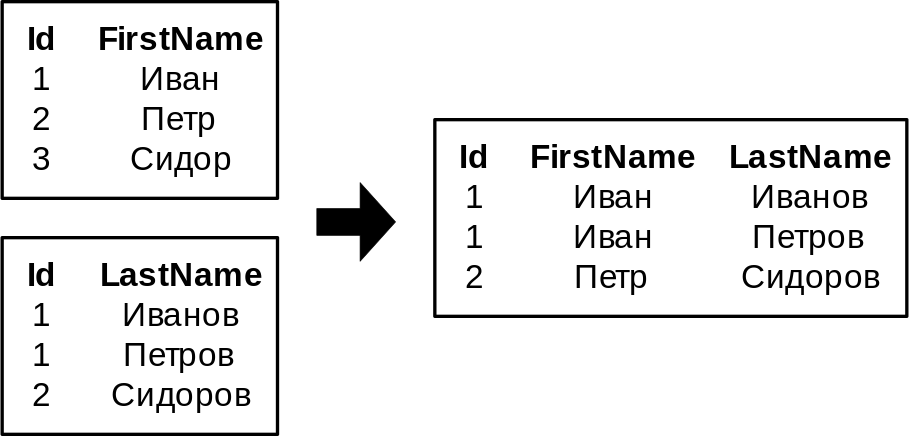
\includegraphics[width=0.8\textwidth]{../assets/kgeorgiy/relalgebra/Join_Natural_2.svg.png}
	\caption{Пример естественного соединения}
	\label{nat-join-ex}
\end{figure}

\paragraph{Размер естественного соединения}

Нетрудно понять, какой минимальный и максимальный размер естественного соединения может получится:
\[
	0 \leqslant \left|R_1 \bowtie R_2 \right| \leqslant |R_1| \times |R_2|.
\] Нижняя оценка достигается при отсутствии равных атрибутов, верхняя -- при
отсутствии общих атрибутов в заголовке.

\subsubsection{Внешнее соединение}

\begin{definition}
	\textit{Внешнее соединение} похоже на естественное (см. \ref{nat-join-def}), только оно сохраняет
	те кортежи, для которых нет соответствующих во втором отношении. Вместо соответствующего берется
	пустой кортеж. Заголовком все так же является объединение заголовков. Обозначение:
	$R_1 \oujoin R_2$.
\end{definition}

На рисунке \ref{outer-join-ex} приведен пример внешнего соединения.

\begin{figure}[H]
	\centering
	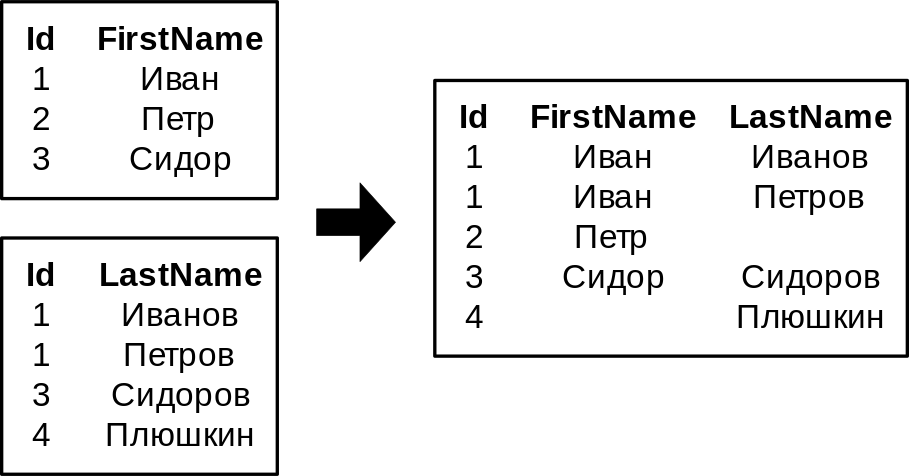
\includegraphics[width=0.8\textwidth]{../assets/kgeorgiy/relalgebra/Join_Outer_2.svg.png}
	\caption{Пример внешнего соединения}
	\label{outer-join-ex}
\end{figure}

\subsubsection{Левое и правое соединения}

\begin{definition}
	\textit{Левым (правым) соединением} называется соединение, аналогичное внешнему, но сохраняющее
	только кортежи из левого (правого) отношения. Обозначается $R_1 \ljoin R_2$
	($R_1 \rjoin R_2$).
\end{definition}

\begin{remark}
	\[
		R_1 \ljoin R_2 \equiv (R_1 \njoin R_2) \cup (R_1 \setminus \pi_{R_1}(R_1 \njoin R_2)),
	\]
	\[
		R_1 \rjoin R_2 \equiv (R_1 \njoin R_2) \cup (R_2 \setminus \pi_{R_2}(R_1 \njoin R_2)).
	\]
	Кроме того, через левое и правое соединения можно выразить внешнее: \[
		R_1 \oujoin R_2 \equiv (R_1 \ljoin R_2) \cup (R_1 \rjoin R_2).
	\]
\end{remark}

На рисунке \ref{lr-join-ex} приведены примеры косых соединений $R_1 \ljoin R_2$ и
$R_1 \rjoin R_2$.

\begin{figure}[H]
	\centering
	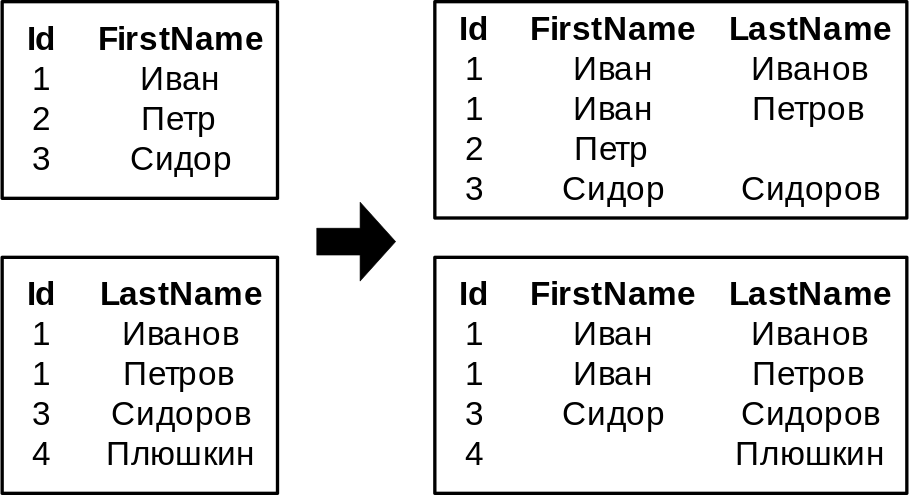
\includegraphics[width=0.8\textwidth]{../assets/kgeorgiy/relalgebra/Join_LeftRight_2.svg.png}
	\caption{Примеры косых соединений}
	\label{lr-join-ex}
\end{figure}

\subsubsection{Полусоединения}

\begin{definition}
	\textit{Левым (правым) полусоединением} называется следующее отношение: $R_1 \lhjoin R_2 \equiv \pi_{R_1}(R_1 \njoin R_2)$
	($R_1 \rhjoin R_2 \equiv \pi_{R_2}(R_1 \njoin R_2)$). Иначе говоря, это отношение, состоящее из
	строк левого (правого) отношения, для которых есть соответствующие строки в правом (левом).
\end{definition}

\begin{remark}
	\enewline
	\begin{itemize}
		\item $R_1 \ljoin R_2 = (R_1 \njoin R_2) \cup (R_1 \setminus R_1 \lhjoin R_2)$.
		\item $R_1 \rjoin R_2 = (R_1 \njoin R_2) \cup (R_2 \setminus R_1 \rhjoin R_2)$.
	\end{itemize}
\end{remark}

На рисунке \ref{lrh-join-ex} приведены примеры полусоединений $R_1 \lhjoin R_2$ и
$R_1 \rhjoin R_2$.

\begin{figure}[H]
	\centering
	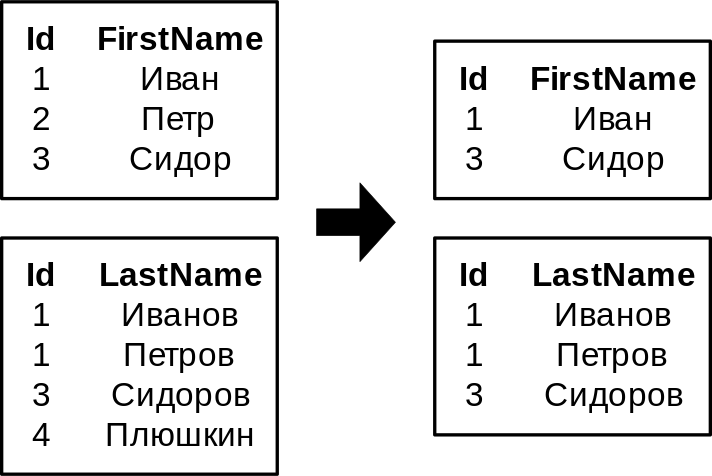
\includegraphics[width=0.8\textwidth]{../assets/kgeorgiy/relalgebra/Join_Semi_2.svg.png}
	\caption{Примеры полусоединений}
	\label{lrh-join-ex}
\end{figure}

\subsubsection{Условные соединения}

\begin{definition}
	Возьмем любое соединение и наложим на него дополнительное условие $\theta$. Получится
	соответствующее условное соединение. Имеется в виду, что нужно отфильтровать результат соединения.
	Однако, не всегда это возможно. Покажем на нескольких примерах, как это должно выглядеть.
	\begin{itemize}
		\item $R_1 \njoin_\theta R_2 = \sigma_\theta(R_1 \njoin R_2)$.
		\item $R_1 \ljoin_\theta R_2 = J \cup (R_1 \setminus \pi_{R_1}(J)),~ J = \sigma_\theta(R_1 \njoin R_2)$.
		\item $R_1 \rjoin_\theta R_2 = J \cup (R_2 \setminus \pi_{R_2}(J)),~ J = \sigma_\theta(R_1 \njoin R_2)$.
		\item $R_1 \oujoin_\theta R_2 = (R_1 \ljoin_\theta R_2) \cup (R_1 \rjoin_\theta R_2)$.
	\end{itemize}
\end{definition}

На рисунке \ref{theta-join-ex} приведен пример левого условного соединения
$R_1 \ljoin_{|FirstName| + 2 < |LastName|} R_2$.

\begin{figure}[H]
	\centering
	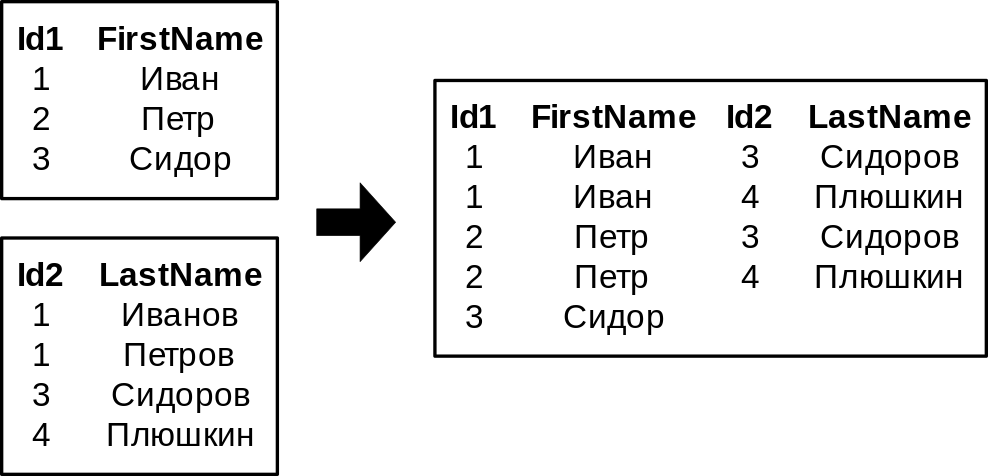
\includegraphics[width=0.8\textwidth]{../assets/kgeorgiy/relalgebra/Join_LeftTheta_2.svg.png}
	\caption{Пример левого условного соединения}
	\label{theta-join-ex}
\end{figure}


\subsection{Реляционная алгебра. Деление и операции над данными}

\subsubsection{Деление}

\begin{definition}
	\textit{Делением}	называется операция, результат которой $R(X) = Q(XY) \div S(Y)$
	максимальный при условии $R \times S \subseteq Q$. Эту операцию можно записать по-другому:
	\begin{itemize}
		\item $Q \div S \equiv \{\,x \mid x \in \pi_X(Q),~ \{x\} \times S \subseteq Q\,\}$.
		\item $Q \div S \equiv \pi_X(Q) \setminus \pi_X(\pi_X(Q) \times S \setminus Q)$.
	\end{itemize}
	Заголовок результирующего отношения -- X. $S \subseteq Q$.
\end{definition}

\begin{remark}
	Интуитивно, эта операция -- запрос всех $X$ таких, что для всех
	$Y$ найдется пара, равная по $X$: $x \in \pi_X(Q)\colon~ \forall y \in S\colon~ (x, y) \in Q$.
\end{remark}

На рисунке \ref{div-ex} представлен пример деления.

\begin{figure}[H]
	\centering
	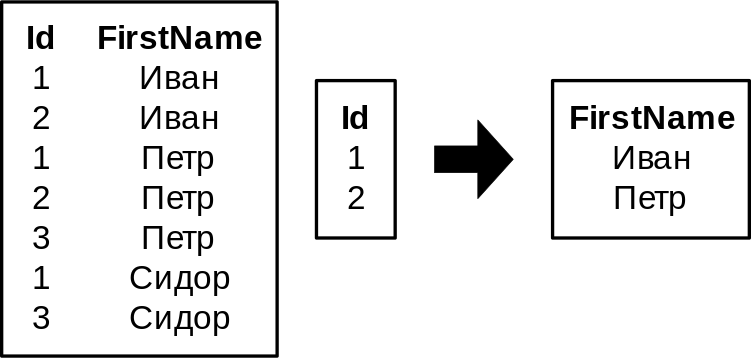
\includegraphics[width=0.8\textwidth]{../assets/kgeorgiy/relalgebra/Divide_Example_2.svg.png}
	\caption{Пример деления}
	\label{div-ex}
\end{figure}

\subsubsection{Большое деление}

\begin{definition}
	\textit{Большим делением} называется операция, которую можно представить следующим образом:
	\begin{itemize}
		\item $Q(XY) \gdiv S(YZ) \equiv \{\,(x, z) \mid \{x\} \times \pi_Y(\sigma_{Z=z}(S)) \subseteq Q \,\}$.
		\item $Q(XY) \gdiv S(YZ) \equiv \pi_X(Q) \times \pi_Z(S) \setminus
			      \pi_{XZ}(\pi_X(Q) \times S \setminus Q \bowtie S)$.
	\end{itemize}
	Заголовок результирующего отношения -- XZ.
\end{definition}

\begin{remark}
	Интуитивно, большое деление -- запрос `для всех связанных', или деление для каждого
	$z$. Иначе говоря, для каждого $z$ найти такие
	$x$, что для всех $y$, связанных с $z$,
	найдется соответсвующий $x$: \[
		(x, z) \in \pi_X(Q) \times \pi_Z(S)\colon~ \forall y \in
		\pi_Y(\sigma_{Z=z}(S))~~ (x, y) \in Q.
	\]
\end{remark}

На рисунке \ref{gdiv-ex} представлен пример большого деления.

\begin{figure}[H]
	\centering
	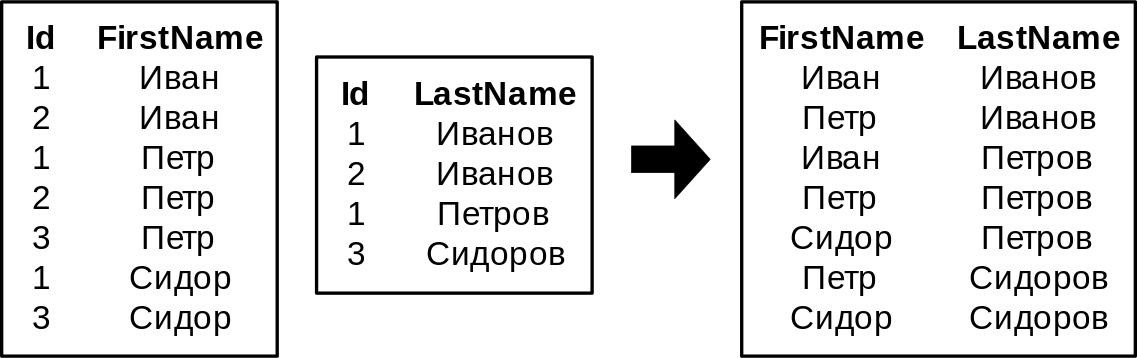
\includegraphics[width=0.8\textwidth]{../assets/kgeorgiy/relalgebra/Divide_Great_Example_2.svg.png}
	\caption{Пример большого деления}
	\label{gdiv-ex}
\end{figure}

\subsubsection{Расширение}

\begin{definition}
	\textit{Расширение} -- операция над данными, добавляющая новый вычисляемый атрибут. Заголовком
	результата будет $R \cup \{A\}$. Обозначение: $\e_{A=\texttt{expr}}(R)$. К каждому кортежу
	тела $R$ добавится вычисленное значение \texttt{expr}. Выражением может
	быть комбинация атрибутов $R$, а также различные функции и операции, доступные в
	БД.
\end{definition}

На рисунке \ref{extend-ex} изображен пример композиции расширений $\e_{\texttt{Tax}=\texttt{tax10(Total)}}
	\circ \e_{\texttt{Total}=\texttt{Price} \cdot \texttt{Items}}$.

\begin{figure}[H]
	\centering
	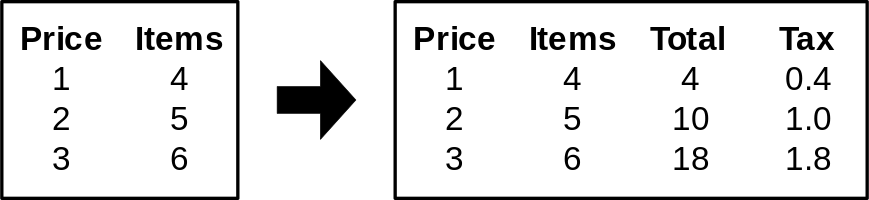
\includegraphics[width=0.8\textwidth]{../assets/kgeorgiy/relalgebra/Data_Extend_2.svg.png}
	\caption{Пример расширения}
	\label{extend-ex}
\end{figure}

\subsubsection{Агрегирование}

\begin{definition}
	\textit{Агрегирование} -- обработка набора значений. Обозначается $\texttt{func}_{Q,A}(R)$.
	\begin{itemize}
		\item Примеры \texttt{func}: \texttt{count, sum, avg, max, min, all, any}.
		\item Q -- агрегируемый атрибут.
		\item A -- сохраняемые атрибуты.
		\item $r \in \pi_A(R)$ расширяется атрибутом $Q = \texttt{func}(\pi_Q\{\,q \in R \mid \pi_A(q) = r\,\})$
	\end{itemize}
\end{definition}

\begin{remark}
	Интуитивно, данные разбиваются по корзинам с одинаковыми $A$, после чего
	каким-то образом сворачиваются,  то есть, на каждой корзине по отдельности считается заданная
	функция.
\end{remark}

На рисунках \ref{aggr-ex-1}, \ref{aggr-ex-2} изображены примеры агрегирования.

\begin{itemize}
	\item $\texttt{sum}_{\texttt{Total},\{\texttt{Supplier}\}} \circ
		      \e_{\texttt{Total}=\texttt{Price} \cdot \texttt{Items}}$
	      \begin{figure}[H]
		      \centering
		      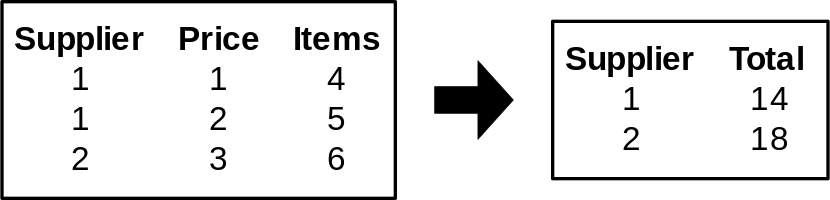
\includegraphics[width=0.8\textwidth]{../assets/kgeorgiy/relalgebra/Data_Aggregate_1_2.svg.png}
		      \caption{Пример агрегирования 1}
		      \label{aggr-ex-1}
	      \end{figure}
	\item $\texttt{sum}_{\texttt{Total},\varnothing} \circ \e_{\texttt{Total}=\texttt{Price} \cdot \texttt{Items}}$
	      \begin{figure}[H]
		      \centering
		      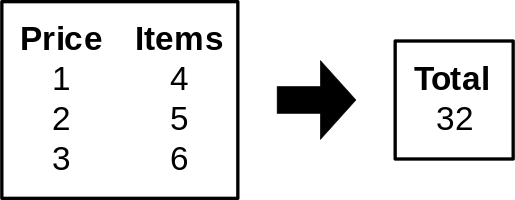
\includegraphics[width=0.8\textwidth]{../assets/kgeorgiy/relalgebra/Data_Aggregate_2_2.svg.png}
		      \caption{Пример агрегирования 2}
		      \label{aggr-ex-2}
	      \end{figure}
\end{itemize}


\subsection{Исчисление кортежей и его реляционная полнота}

\subsubsection{Реляционное исчисление}

\begin{definition}
	\textit{Реляционное исчисление} -- декларативный язык для работы с отношениями.
\end{definition}

В отличие от реляционной алгебры, в реляционном исчислении описывается не то, как построить запрос,
а свойства результата, который ожидаем получить.

Выделяют два вида реляционного исчисления: \textbf{исчисление кортежей} и \textbf{исчисление доменов}.

\paragraph{Части запроса}

\begin{itemize}
	\item \textbf{Определение переменных},
	\item \textbf{Определение свойств результата}.
\end{itemize}

\paragraph{Синтаксис запроса}

\begin{lstlisting}[language=SQL]
    <variables definition>
    select <attributes list>
    from <variables>
    where <condition>
\end{lstlisting}

\paragraph{Пример}

Рассмотрим запрос, для получения идентификаторов студентов, обучающихся в группе
\texttt{M34371}.

Запрос в реляционной алгебре:

\[
	\pi_{SId}(\sigma_{Name = M34371} (Students \bowtie Groups))
\]

Запрос в реляционном исчислении:

\begin{lstlisting}[language=SQL, mathescape=true]
    select S.SId from S
    where $\exists$ G (S.GId = G.GId $\wedge$ G.Name = 'M34371')
\end{lstlisting}

\subsubsection{Исчисление кортежей}

В качестве переменных выступают кортежи. Тип переменной определяется именем и типами атрибутов, а
также набором значений. Заметим, что это есть отношение.

\paragraph{Синтаксис}

\begin{lstlisting}
    <Variable> :: <Relation>
\end{lstlisting}

\paragraph{Операции с отношениями}

\begin{itemize}
	\item \textbf{Огранричение}
	      \begin{lstlisting}[language=SQL]
    <Relation> where <Condition>
        \end{lstlisting}
	\item \textbf{Объединение}
	      \begin{lstlisting}[language=SQL]
    <Relation 1>, <Relation 2>
        \end{lstlisting}
\end{itemize}

\paragraph{Примеры}

Рассмотренное выше отношение \texttt{G4} можно выразить иначе:

\begin{lstlisting}[language=SQL, mathescape=true]
    G4 :: Groups where Name = 'M34351',
          Groups where Name = 'M34371',
          Groups where Name = 'M34391'
\end{lstlisting}

\paragraph{Условия}

Условия во многом аналогичны условиям из реляционной алгебры. Дополнительно вводятся кванторы.

\begin{itemize}
	\item \textbf{Простые условия}.
	      \begin{itemize}
		      \item Сравнение атрибутов с константами
		            \begin{lstlisting}[language=SQL, mathescape=true]
    S.Name = 'John'
    S.Id $<$ 5
                \end{lstlisting}
		      \item Сравнение атрибутов между собой
		            \begin{lstlisting}[language=SQL, mathescape=true]
    S.Id $\geq$ G.Id
                \end{lstlisting}
		      \item Сравнение с применением формул
		            \begin{lstlisting}[language=SQL, mathescape=true]
    length(S.FirstName) = length(S.LastName) + 3
                \end{lstlisting}
	      \end{itemize}
	\item \textbf{Составные условия}. Вводятся логические связки: $\vee$, $\wedge$,
	      $\neg$.
	      \begin{lstlisting}[language=SQL, mathescape=true]
    G where Name = 'M34371' $\vee$ Name = 'M34391'
    S where FirstName = 'John' $\wedge$ LastName <> 'Smith'
        \end{lstlisting}
	\item \textbf{Условия с кванторами}. Вводятся кванторы всеобщности $\forall$ и существования
	      $\exists$. Синтаксис: \texttt{<quantifier> <variable> (<condition>)}.
	      \begin{lstlisting}[language=SQL, mathescape=true]
    G where $\exists$ S (S.FirstName = 'John' $\wedge$ S.GId = G.GId)
    G where $\forall$ S (S.FirstName = 'John' $\vee$ S.GId = G.GId)
        \end{lstlisting}
\end{itemize}

\paragraph{Примеры}

Рассмотрим примеры введения переменных, запроса, который требует в реляционной алгебре применения
деления, и работы с несколькими отношениями.

\begin{lstlisting}[language=SQL, mathescape=true]
    -- Variables declaration
    S :: Students; G :: Groups; C :: Courses; P :: Point;
    G4 :: Groups where Name = 'M34351' $\vee$
        Name = 'M34371' $\vee$ Name = 'M34391'

    -- Fully marked groups
    select G.GId from G where $\forall$ S ($\forall$ C($\exists$ P
        (S.Sid = P.Sid $\wedge$ C.CId = P.CId $\wedge$ P.Points $\geq$ 60)))

    -- Multiple relations
    select S.FirstName, S.LastName, G.Name
    from S, G
    where S.GId = G.GId
\end{lstlisting}

\subsubsection{Связи реляционной алгебры и исчисления кортежей}

\paragraph{Алгебра через исчисление}

Выразим реляционную алгебру через исчисление кортежей.

\begin{itemize}
	\item \textbf{Проекция}.
	      \begin{itemize}
		      \item $\pi_{A_1, \ldots, A_n}(R)$
		      \item \texttt{select A1, ..., An from R}
	      \end{itemize}
	\item \textbf{Фильтрация}.
	      \begin{itemize}
		      \item $\sigma_{\theta}(R)$
		      \item \texttt{from R where $\theta$}
	      \end{itemize}
	\item \textbf{Создание нового столбца}.
	      \begin{itemize}
		      \item $\epsilon_{A=expr}(R)$
		      \item \texttt{select R.*, expr as A from R}
	      \end{itemize}
	\item \textbf{Объединение}.
	      \begin{itemize}
		      \item $R_1 \cup R_2$
		      \item \texttt{R :: R1, R2}
	      \end{itemize}
	\item \textbf{Разность}.
	      \begin{itemize}
		      \item $R_1 \setminus R_2$
		      \item \texttt{R :: R1 where $\neg \exists$ R2 (R1 = R2)}
	      \end{itemize}
	\item \textbf{Декартово произведение}.
	      \begin{itemize}
		      \item $R_1 \times R_2$
		      \item \texttt{select R1.*, R2.* from R1, R2}
	      \end{itemize}
	\item \textbf{Объединение}.
	      \begin{itemize}
		      \item $R_1 \bowtie R_2$
		      \item \texttt{select R1.*, R2.* from R1, R2}
		            \linebreak \texttt{where R1.<common\_attrs> = R2.<common\_attrs>}
	      \end{itemize}
\end{itemize}

Указанные выше операции образуют базис реляционной алгебры. Следовательно, выразительная мощность
реляционной алгебры \textit{не больше} выразительной мощности реляционного исчисления, и
алгебру можно выразить через исчисление.

\paragraph{Исчисление через алгебру}

Выражения с кванторами можно привести к предваренной нормальной форме (сначала идут только
кванторы, затем -- условие). После этого можно преобразовать выражение в алгебру:

\begin{itemize}
	\item Построение выражения для каждой переменной,
	\item Построение декартового произведения по всем затронутым отношениям,
	\item Фильтрация по условию,
	\item Применение кванторов:
	      \begin{itemize}
		      \item Квантор существования: проекция, исключая атрибуты, порожденные переменной. Если существует хотя бы
		            одно значение кортежной переменной, удовлетворяющее условию, то проекция будет непустой. Верно
		            обратное.
		      \item Квантор всеобщности: как было замечено, логике этого квантора соответствует деление. Таким образом,
		            достаточно делить на все столбцы кортежной переменной.
	      \end{itemize}
\end{itemize}

\paragraph{Пример}

Запрос получает идентификаторы групп, в которых есть хотя бы один студент, аттестованный по всем
дисциплинам.

\begin{lstlisting}[language=SQL, mathescape=true]
    select G.GId where $\exists$ S($\forall$ C($\exists$ P
        (G.GId = S.GId $\wedge$ S.SId = P.SId $\wedge$
         C.CId = P.CId $\wedge$ P.Points $\geq$ 60)))
\end{lstlisting}

Преобразуем его в реляционную алгебру.

\[
	T_0 = \sigma_{P.Points \geq 60}((G \bowtie S \times C) \bowtie P)
\]

Самый внутренний квантор ($\exists P$) -- проекция на все внешние атрибуты (находящиеся
левее в выражении):

\[
	T_1 = \pi_{G_*, S_*, C_*}(T_0)
\]

Далее следует квантор всеобщности ($\forall C$) -- деление на переменную:

\[
	T_2 = T_1 \div C
\]

Последний квантор существования ($\exists S$) -- проекция на единственный оставшийся
внешний атрибут:

\[
	T_3 = \pi_{G_*}(T_2)
\]

Получили выражение в терминах реляционной алгебры:

\[
	T = \pi_{G_*}(\pi_{G_*, S_*, C_*} (\sigma_{P.Points \geq 60}((G \bowtie S \times C) \bowtie P))
	\div C)
\]

\begin{proposition}
	Выразительная мощность исчисления кортежей равна выразительной мощности реляционной алгебры.
\end{proposition}

\begin{definition}
	\textit{Реляционно-полные языки} -- языки, выразительная мощность которых не меньше
	выразительной мощности реляционной алгебры.
\end{definition}

Следовательно, исчисление кортежей -- реляционно-полный язык.

\subsection{Исчисление доменов и его реляционная полнота}

\subsubsection{Исчисление доменов}

В качестве переменных выступают домены (типы). Иными словами, работа ведется с атомарными
переменными в отличие от исчисления кортежей, где работа ведется с отношениями.

\paragraph{Синтаксис объявления переменных}

Указывается имя и \textit{домен (тип)}.

\begin{lstlisting}
    <Variable> :: <Type>
\end{lstlisting}

\paragraph{Пример}

Можно использовать типы из SQL.

\begin{lstlisting}[language=SQL]
    SId :: Int
    FirstName :: Varchar(100)
\end{lstlisting}

\paragraph{Условие принадлежности}

Для связи доменов с отношениями вводится предикат проверки принадлежности значения заданному
кортежу.

\paragraph{Синтаксис}

Отсутствие какого-либо атрибута отношения означает, что его конкретное значение нас не интересует.

\begin{lstlisting}[language=SQL]
    <Relation> {
        <Attribute1> = <Value1>,
        <Attribute2> = <Value2>,
        ...
    }
\end{lstlisting}

\paragraph{Пример}

В последнем примере \texttt{SId = SId} означает, что аттрибут \texttt{SId} (слева) равен
значению переменной с именем \texttt{SId}. Не отличается по смыслу от предыдущего.

\begin{lstlisting}[language=SQL]
    S{FirstName = 'John', LastName = 'Smith'}
    S{SId = Id}
    S{SId = SId}
\end{lstlisting}

\paragraph{Примеры}

\begin{itemize}
	\item Идентификаторы всех студентов:
	      \begin{lstlisting}[language=SQL]
    SId where S{SId = SId}
        \end{lstlisting}
	\item Идентификаторы всех студентов определенной группы:
	      \begin{lstlisting}[language=SQL]
    SId where S{SId = SId, GId = 'M34371'}
        \end{lstlisting}
	\item Идентификаторы всех студентов двух определенных групп:
	      \begin{lstlisting}[language=SQL, mathescape=true]
    SId where S{SId = SId, GId = 'M34371'} $\vee$
              S{SId = SId, GId = 'M34391'}
        \end{lstlisting}
	\item Идентификаторы всех студентов, не сдавших курс с определенным идентификатором.
	      \begin{lstlisting}[language=SQL, mathescape=true]
    SId where $\neg \exists$ Points (Points $\geq$ 60 $\wedge$
        P {SId = SId, Points = Points, CId = 10})
        \end{lstlisting}
\end{itemize}

\subsubsection{Связи реляционной алгебры и исчисления доменов}

\paragraph{Алгебра через исчисление}

Выразим реляционную алгебру через исчисление доменов.

\begin{itemize}
	\item \textbf{Проекция}.
	      \begin{itemize}
		      \item $\pi_{A_1, \ldots, A_n}(R)$
		      \item \texttt{A1, ..., An from R where R\{A1 = A1, ..., An = An\}}
	      \end{itemize}
	\item \textbf{Фильтрация}.
	      \begin{itemize}
		      \item $\sigma_{\theta}(R)$
		      \item \texttt{A1, ..., An from R where R\{A1 = A1, ..., An = An\} $\wedge$ $\theta$}
	      \end{itemize}
	\item \textbf{Создание нового столбца}.
	      \begin{itemize}
		      \item $\epsilon_{A=expr}(R)$
		      \item \texttt{expr as A from R where R\{A1 = A1, ..., An = An\}}
	      \end{itemize}
	\item \textbf{Объединение}.
	      \begin{itemize}
		      \item $R_1 \cup R_2$
		      \item \texttt{A1, ..., An where R1\{..., Ai = Ai, ...\} $\vee$ R2\{..., Ai = Ai, ...\}}
	      \end{itemize}
	\item \textbf{Разность}.
	      \begin{itemize}
		      \item $R_1 \setminus R_2$
		      \item \texttt{A1, ..., An where R1\{..., Ai = Ai, ...\} $\vee$ $\neg$
			            R2\{..., Ai = Ai, ...\}}
	      \end{itemize}
	\item \textbf{Декартово произведение}.
	      \begin{itemize}
		      \item $R_1 \times R_2$
		      \item \texttt{A1, ..., An, B1, ..., Bm where R1\{..., Ai = Ai, ...\} $\wedge$}
		            \linebreak \texttt{R2\{..., Bj = Bj, ...\}}
	      \end{itemize}
	\item \textbf{Объединение}.
	      \begin{itemize}
		      \item $R_1 \bowtie R_2$
		      \item \texttt{A1, ..., An, B1, ..., Bm, C1, ..., Cl}
		            \linebreak \texttt{where R1\{..., Ai = Ai, ..., Bj = Bj, ...\} $\wedge$}
		            \linebreak \texttt{R2\{..., Bj = Bj, ..., Ck = Ck, ...\}}
	      \end{itemize}
\end{itemize}

\begin{proposition}
	Выразительная мощность исчисления доменов не меньше выразительной мощности реляционной алгебры, то
	есть исчисление доменов -- реляционно-полный язык.
\end{proposition}

\subsection{Datalog и рекурсия}

\subsubsection{Datalog}

\textit{Datalog} -- язык запросов к БД. Разработан в 1978 году, имеет много схожего с языком
Prolog. Повлиял
на развитие SQL. Реализует исчисление доменов.

Программа на языке состоит из набора определений отношений. Результатом считается тело одного из
отношений.

\paragraph{Конструкции языка}

\begin{itemize}
	\item \textbf{Реляционные атомы}. Реализуют предикат вхождения из исчисления доменов.
	      Используется позиционная запись аргументов.
	      \begin{lstlisting}[mathescape=true]
    -- Values belong to relation R
    R(x1, x2, ..., xn)
    -- Values do not belong to relation R
    $\neg$ R(x1, x2, ..., xn)
        \end{lstlisting}
	\item \textbf{Арифметические атомы}. Сравнение двух выражений.
\end{itemize}

\paragraph{Синтаксис}

Программа состоит из списка строк:

\begin{lstlisting}
    <Relation>(<Attr 1>, <Attr 2>, ..., <Attr n>) :- <Target>
\end{lstlisting}

Цель (target) -- последовательность атомов. В отношение (Relation) входят кортежи, удовлетворяющие
хотя бы одной цели (всем атомам хотя бы одной цели).

Иначе говоря, запросы пишутся в дизъюнктивной нормальной форме.

\paragraph{Примеры}

\begin{itemize}
	\item Идентификаторы и фамилии всех студентов с заданным именем:
	      \begin{lstlisting}
    Johns(Id, LastName) :-
        Students(Id, FirstName, LastName),
        FirstName = 'John'.
        \end{lstlisting}
	\item Имена всех студентов и преподавателей:
	      \begin{lstlisting}
    Names(Name) :- Students(_, Name, _).
    Names(Name) :- Lecturers(_, Name, _).
        \end{lstlisting}
\end{itemize}

\paragraph{Бесконечные отношения}

Запросы могут породить бесконечные отношения. Например:

\begin{lstlisting}[mathescape=true]
    NotStudent(Id, Name) :- $\neg$ Students(Id, Name, _).
\end{lstlisting}

Здесь нет ограничения на фамилию студента -- ни по типу, ни по значению -- поэтому это отношение
бесконечно и содержит студентов с почти произвольными фамилиями.

\begin{proposition}
	Для запрета бесконечных отношения достаточно принудить каждую переменную входить как минимум в один
	неотрицательный реляционный атом.
\end{proposition}

\paragraph{Реляционная алгебра через Datalog}

Выразим реляционную алгебру через исчисление доменов.

\begin{itemize}
	\item \textbf{Проекция}.
	      \begin{itemize}
		      \item $\pi_{A_1, \ldots, A_n}(R)$
		      \item \texttt{Q(A1, ..., An) :- R(A1, ..., An, \_, ..., \_).}
	      \end{itemize}
	\item \textbf{Фильтрация}.
	      \begin{itemize}
		      \item $\sigma_{\theta}(R)$
		      \item \texttt{Q(A1, ..., An) :- R(A1, ..., An, \_, ..., \_), $\theta$.}
	      \end{itemize}
	\item \textbf{Объединение}.
	      \begin{itemize}
		      \item $R_1 \cup R_2$
		      \item \texttt{Q(A1, ..., An) :- R1(A1, ..., An).}
		            \linebreak \texttt{Q(A1, ..., An) :- R2(A1, ..., An).}
	      \end{itemize}
	\item \textbf{Разность}.
	      \begin{itemize}
		      \item $R_1 \setminus R_2$
		      \item \texttt{Q(A1, ..., An) :- R1(A1, ..., An), $\neg$ R2(A1, ..., An).}
		      \item \textbf{Замечание}. Запись корректна, поскольку атрибуты \texttt{A1, ..., An} входят
		            в неотрицательный реляционный атом R1.
	      \end{itemize}
	\item \textbf{Декартово произведение}.
	      \begin{itemize}
		      \item $R_1 \times R_2$
		      \item \texttt{Q(A1, ..., An, B1, ..., Bm) :- R1(A1, ..., An), R2(B1, ..., Bm).}
	      \end{itemize}
	\item \textbf{Объединение}.
	      \begin{itemize}
		      \item $R_1 \bowtie R_2$
		      \item \texttt{Q(A1, ..., An, B1, ..., Bm, C1, ..., Cl) :-}
		            \linebreak \texttt{R1(A1, ..., An, B1, ..., Bm), R2(B1, ..., Bm, C1, ..., Cl).}
	      \end{itemize}
\end{itemize}

\begin{proposition}
	Datalog -- реляционно-полный язык.
\end{proposition}

\begin{remark}
	В Datalog нет явных кванторов. Есть только неявный квантор существования -- для свободных
	переменных справа в выражении.
\end{remark}

\paragraph{Пример}

Рассмотрим таблицу:

\begin{lstlisting}
    Person(Id, Name, MotherId, FatherId)
\end{lstlisting}

Получить для каждого человека имена обоих родителей:

\begin{lstlisting}
    Parents(N, FN, MN) :- Person(_, N, FId, MId),
        Person(FId, FN, _, _), Person(MId, MN, _, _).
\end{lstlisting}

Получить для каждого человека имя его родителя:

\begin{lstlisting}
    Parents(N, FN) :- Person(_, N, FId, _), Person(FId, FN, _, _).
    Parents(N, MN) :- Person(_, N, MId, _), Person(MId, MN, _, _).
\end{lstlisting}

\subsubsection{Рекурсивные запросы}

Datalog позволяет строить рекурсивные запросы, например, для транзитивного замыкания. Рассмотрим
для примера таблицу:

\begin{lstlisting}
    Parent(Id, ParentId)
\end{lstlisting}

И запрос для получения всех предков (представляющий собой транзитивное замыкание):

\begin{lstlisting}
    Ancestor(Id, PId) :- Parent(Id, PId).
    Ancestor(Id, GId) :- Parent(Id, PId), Ancestor(PId, GId).
\end{lstlisting}

Такому запросу отвечает несколько множеств кортежей. Формально, помимо ожидаемого транзитивного
замыкания, декартово произведение всех возможных идентификаторов будет удовлетворять запросу. При
этом, такое множество кортежей будет \textit{неподвижной точкой} -- множеством, которое нельзя дополнить
по правилам вывода. Но такой результат не будет иметь практического смысла

Во избежание неопределенности, в Datalog результатом рекурсивного запроса является
\textit{минимальная неподвижная точка} -- минимальное по включению множество, такое что левая и правая части
совпадают.

На практике рекурсивное правило применяется, пока не будет достигнута неподвижная точка. Очевидно,
она будет минимальной по включению.

\paragraph{Поиск минимальной неподвижной точки}

\begin{itemize}
	\item Инициализация нерекурсивными данным,
	\item Пока есть следствия, данные  пополняются ими.
\end{itemize}

\begin{remark}
	Отрицания в рекурсивных правилах могут приводить к парадоксам (например, на шаге
	$n$ какие-то данные должны быть добавлены, на $n + 1$ -- нет).
	Поэтому в рекурсивных запросах явно запрещены циклы, содержащие отрицания.
\end{remark}

\begin{remark}
	Как было замечено ранее, реляционная алгебра не позволяет построить рекурсивные запросы.
	Следовательно, выразительная мощность Datalog больше, чем у реляционной алгебры.
\end{remark}

\subsubsection{Связь реляционного исчисления и SQL}

\begin{itemize}
	\item \textbf{Заголовок запроса}. Определяет, какие данные будут получены. В реляционной
	      алгебре соответствует самой внешней проекции. В реляционном исчислении -- заголовку запроса.
	\item \textbf{Раздел \texttt{from}}. Определяет набор отношений, с которыми производится
	      работа. В реляционной алгебре здесь указываются соединения. В реляционном исчислении -- переменные
	      отношений.
	\item \textbf{Раздел \texttt{where}}. Определяет набор отношений, с которыми производится
	      работа. В реляционной алгебре соответствует самой внешней фильтрации. В реляционном исчислении --
	      условию на кортежи.
\end{itemize}

\begin{remark}
	В языке SQL на практике большинство кванторов применяется для соединений. Однако, существует также
	явный квантор существования. Как было показано в Datalog, квантор всеобщности избыточен
	($\forall v(p(v)) \equiv \neg \exists v(\neg p(v))$)
\end{remark}

\subsubsection{Подзапросы}

Квантор существования предоставлен в SQL через подзапросы существования:

\begin{itemize}
	\item Существования (\texttt{exists}),
	\item Вхождения (\texttt{in}),
	\item Условные (\texttt{any, all}),
	\item Скалярные.
\end{itemize}

\paragraph{Подзапрос существования}

Если подзапросу удовлетворяет хотя бы один кортеж, то оператор возвращает \texttt{true},
иначе \texttt{false}.

\begin{lstlisting}[language=SQL]
    [not] exists (select ...)
\end{lstlisting}

\paragraph{Пример}

Группы, в которых нет студентов:

\begin{lstlisting}[language=SQL]
    select G.Name where
    not exists (select * from S where S.Gid = G.Gid)
\end{lstlisting}

\paragraph{Подзапрос вхождения}

Если результаты всех выражений входят в подзапрос, то оператор возвращает \texttt{true},
иначе \texttt{false}.

\begin{lstlisting}[language=SQL]
    (<list of expressions>) [not] in (select ...)
\end{lstlisting}

\begin{remark}
	Многие СУБД поддерживают подзапросы только с одним столбцом.
\end{remark}

\paragraph{Пример}

Оценки по предметам 4 курса:

\begin{lstlisting}[language=SQL]
    select * from P where P.CId in
        (select CId from C where Year = 4)
\end{lstlisting}

\paragraph{Условный подзапрос}

\texttt{any} возвращает \texttt{true}, если для одного из значений выполняется
условие. Аналогично,
\texttt{all} возвращает \texttt{true}, если для всех значений выполняется
условие.

\begin{lstlisting}[language=SQL]
    <expression> <condition> { any | all } (select ...)
\end{lstlisting}

\paragraph{Пример}

Лучшие студенты по предметам:

\begin{lstlisting}[language=SQL]
    select SId, CId from P as PE where PE.Points >=
        all (select Points from P where P.CId = PE.CId)
\end{lstlisting}

\paragraph{Скалярные подзапросы}

Запросы, возвращающие не более одного значения.

\begin{lstlisting}[language=SQL]
    (select ...)
\end{lstlisting}

\begin{remark}
	Результатом скалярного подзапроса, вернувшего пустой результат, является \texttt{null}.
\end{remark}

\paragraph{Пример}

Студенты и название группы:

\begin{lstlisting}[language=SQL]
    select
        SId,
        (select Name from G where G.GId = S.GId)
    from S
\end{lstlisting}

\paragraph{Кореллированные подзапросы}

\begin{definition}
	Подзапрос называется \textit{кореллированным (некореллированным)}, если в нем есть (отсутствуют) свободные переменные.
\end{definition}

\paragraph{Примеры}

Лучшие студенты по предметам (кореллированный подзапрос, \texttt{PE} -- свободная
переменная):

\begin{lstlisting}[language=SQL, escapechar=\%]
    select SId, CId from P as %\underline{PE}% where PE.Points >=
        all (select Points from P where P.CId = %\underline{PE}%.CId)
\end{lstlisting}

Оценки по предметам четвертого курса (некореллированный подзапрос):

\begin{lstlisting}[language=SQL]
    select * from P where P.CId in
        (select CId from C where Year = 4)
\end{lstlisting}

\begin{remark}
	Преимущество некореллированных подзапросов в том, что их можно посчитать один раз и
	переиспользовать результат в дальнейшем. Поэтому на практике они предпочтительнее кореллированных.
\end{remark}

\subsubsection{Рекурсия}

Поддержка рекурсии была добавлена в SQL3. Однако, многие СУБД не поддерживают ее.

\paragraph{Синтаксис}

Как и в Datalog, отрицание должно быть стратифицировано -- оно запрещено в циклах рекурсии.

\begin{lstlisting}[language=SQL]
    with recursive <relation>(<columns>) as ...
\end{lstlisting}

\paragraph{Пример}

Транзитивное замыкание предков:

\begin{lstlisting}[language=SQL]
    with recursive Ancestor(Id, AId) as
        select Id, PId from Parent
        union
        select P.Id, AId from Ancestor a
            inner join Parent p on a.Id = p.PId
    select * from Ancestor
\end{lstlisting}

\subsection{Транзакции. Восстановление. Классический алгоритм}

\subsubsection{Транзакции}

\begin{definition}
	\textit{Транзакция} -- минимальный объем работы, который можно
	зафиксировать в базе данных.
\end{definition}

Каждый оператор заключен в неявную транзакцию, которая начинается непосредственно перед оператором
и заканчивается после него. Не все действия в СУБД являются транзакционными. Например, во многих
реализациях не поддерживается транзакционное изменение схемы данных.

\paragraph{Свойства транзакций (ACID)}

\begin{definition}
	\textit{Атомарность (Atomicity)} -- с точки зрения БД, транзакция либо
	выполняется целиком, либо полностью откатывается. Иначе говоря, никто со стороны не может увидеть
	промежуточное состояние выполнения транзакции.
\end{definition}

\begin{definition}
	\textit{Согласованность (Consistency)} -- после завершения транзакции БД
	остается в согласованном состоянии.
\end{definition}

\begin{definition}
	\textit{Изоляция (Isolation)} -- транзакции не могут взаимодействовать
	между собой. Это означает, что транзакции не могут пользоваться промежуточными результатами друг
	друга.
\end{definition}

\begin{definition}
	\textit{Устойчивость (Durability)} -- при успешном завершении транзакции
	результаты ее исполнения сохраняются в БД, при откате транзакции все внесенные ею изменения
	отменяются.
\end{definition}

\paragraph{Корретность и согласованность}

\begin{definition}
	Состояние БД является \textit{согласованным}, если оно удовлетворяет всем объявленным ограничениям.
	Это свойство автоматически проверяется СУБД.
\end{definition}

\begin{definition}
	Состояние БД является \textit{корректным}, если оно соответствует реальному миру. Автоматически
	проверено быть не может.
\end{definition}

Существуют условия корректности, которые нельзя проверить ограничениями. Например, после перевода
денег в банке их общая сумма в системе не должна измениться. Однако, эта сумма заранее неизвестна,
поэтому заранее задать ограничение невозможно.

\paragraph{Минимизация транзакций}

Транзакции требуют большие ресурсные затраты, поэтому должны быть минимальными. По возможности
следует использовать неявные транзакции.

Однако, есть типичные ситуации, в которых использования неявных транзакций недостаточно:

\begin {itemize}
\item \textit{Условное обновление} -- проверку условия и обновление
необходимо сделать в рамках одной транзакции, в противном случае в момент изменения условие может
перестать выполняться; \item \textit{Множественное обновление} -- при обновлении данных, особенно в различных
таблицах, использование транзакции необходимо для исключения несогласованности; \item
\textit{Промежуточная несовместимость} -- некоторые действия требуют временного нарушения согласованности с
последующим его восстановлением, использование транзакций позволяет откладывать проверку
согласованности до завершения всех действий и исключают видимость несогласованного состояния
другими пользователями. \end {itemize}

Также следует отметить, что результат завершения транзакции \textbf{не должен зависеть от человека}. Человеческий
фактор может привести к зависшей транзакции. Если требуется принятие решения от человека,
транзакцию следует разбить на две: первая читает данные, а вторая их записывает, предварительно
проверяя данные на соответствие результату первой. В таком случае от решения человека зависит
применение второй транзакции.

\subsubsection{Восстановление}

Напомним, что свойство \textit{устойчивости (durability)} транзакции подразумевает сохранение результатов
транзакции в БД даже при сбоях.

Хранение данных в оперативной памяти может приводить к потерям, например, при перезагрузке. Это
считается нормальным, что приводит к необходимости хранения информации на дисках. Напомним, что с
диска быстрее читать данные последовательно.

\paragraph{Типы сбоев}

\begin{itemize}
	\item \textbf{Локальный}. Сбой одной транзакции. Для восстановления
	      достаточно откатить затронутую транзакцию.
	\item \textbf{Глобальный}. Сбой процесса СУБД, затрагивает все транзакции.
	      Для восстановления достаточно откатить все незавершенные транзакции, а также заново применить все
	      успешно завершенные транзакции.
	\item \textbf{Аппаратный}. Например, перезагрузка компьютера. С точки
	      зрения СУБД, не существенно отличается от глобального сбоя.
	\item \textbf{Отказ оборудования}. СУБД не может восстановиться после этого
	      типа сбоя. Однако, многие СУБД предоставляют \textit{средства} для восстановления (например,
	      запись данных на несколько дисков и синхронизация копий).
\end{itemize}

Свойство устойчивости не является абсолютным. Существуют сбои, при которых его нельзя поддержать.

\paragraph{Восстановление после сбоя}

Для восстановления БД достаточно сделать следующее:

\begin{itemize}
	\item Успешные транзакции -- зафиксировать;
	\item Откаченные транзакции -- откатить;
	\item Незавершенные транзакции -- откатить.
\end{itemize}

Существует несколько популярных подходов для отката:

\paragraph{Shadow copy}

Каждая транзакция пишет данные в новое место. При успешном завершении транзакции копия помечается
успешной, пользователь уведомляется об успешной транзакции, и начинается запись из копии в БД. При
сбое во время записи производится повторная запись. Проблема подхода заключается в частых чтениях и
записях shadow copy, которые расположены в случайных местах на диске, что медленно.

\paragraph{Transaction log}

Данные пишутся сразу в БД, параллельно записывая изменения, примененные в рамках каждой транзакции,
в журнал. Данный подход более популярен.

Журнал записывается в надежное хранилище изменений. Это означает, что его утрата есть
невосстановимый сбой. Однако, записи ведутся последовательно, что делает данный подход быстрее
предыдущего.

В журнал записываются: старые данные, новые данные, маркеры начала и завершения транзакции.

При завершении транзакции все изменения записываются в журнал, записывается маркер завершения
транзакции, пользователь уведомляется о завершении транзакции.

\paragraph{Реализация журнала}

\begin{itemize}
	\item \textbf{Постоянная запись на диск}. При записи каждого изменения в
	      журнал существенно возрастает число операций, конкуренция за доступ к диску, а также накапливаются
	      откаченные транзакции, которые в будущем не принесут пользы.
	\item \textbf{Запись при завершении}. В журнал при завершении транзакции
	      записываются порожденные изменения. При больших изменениях это приводит к росту потребления памяти
	      журналом.
	\item \textbf{Точки восстановления}. В журнал периодически записывается
	      "слепок" состояния системы: текущие изменения, завершенные транзакции
	      (не записанные ранее), откаченные транзакции (не записанные ранее),
	      открытые транзакции. Создание точки восстановления требует приостановки изменений.
\end{itemize}

\paragraph{Структура журнала}

С использованием механизма точек восстановления, получаем следующую структуру журнала.

\begin{itemize}
	\item \textbf{Точка восстановления};
	\item \textbf{События}:
	      \begin{itemize}
		      \item Идентификатор транзакции,
		      \item Указатель на \textit{предыдущее} событие транзакции:
		            \begin{itemize}
			            \item Начало транзакции,
			            \item Изменение,
			            \item Завершение транзакции,
			            \item Откат транзакции.
		            \end{itemize}
	      \end{itemize}
\end{itemize}

\paragraph{Примеры}
Рассмотрим пример сбоя и определим, что должно произойти с каждой из транзакций.

\begin{figure}[h]
	\centering
	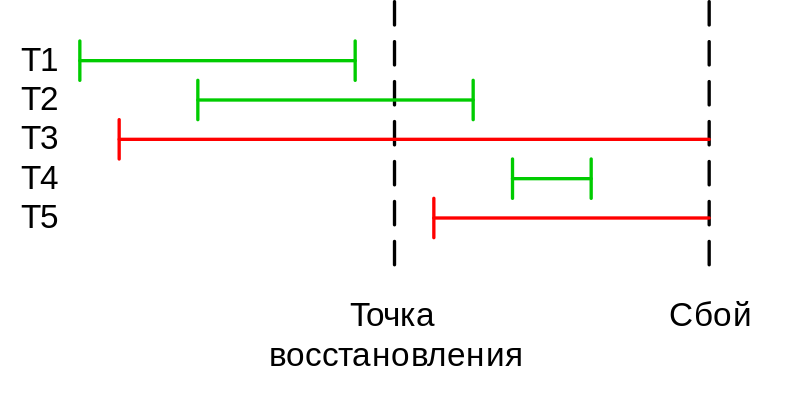
\includegraphics[width=0.8\textwidth]{../assets/kgeorgiy/transactions/Recovery_TransactionLog_2.svg.png}
	\caption{Иллюстрация к определению проекции}
	\label{tx-log}
\end{figure}

Зеленым и красным цветом отмечены транзакции, которые должны быть завершены или откачены
соответственно при восстановлении. Отметим, что эти решения однозначно определены гарантиями ACID
транзакций.

\subsubsection{Классический алгоритм восстановления}

\paragraph{Фазы алгоритма}

\begin{itemize}
	\item \textbf{Разметка транзакций}. Каждая транзакция отмечается как
	      \textit{Redo} или \textit{Undo}.
	\item \textbf{Откат транзакций}. Для помеченных как \textit{Undo}.
	\item \textbf{Повтор транзакций}. Для помеченных как \textit{Redo}.
\end{itemize}

\paragraph{Фаза разметки транзакций}

\begin{itemize}
	\item Чтение журнала идет от последней точки восстановления до конца. Все открытые транзакции помещаются
	      в \textit{Undo}.
	\item При чтении маркера начала транзакция добавляется в \textit{Undo}.
	\item При чтении маркера конца транзакция переносится из \textit{Undo} в \textit{Redo}.
\end{itemize}

\paragraph{Фаза отката транзакций}

\begin{itemize}
	\item Чтение журнала идет от конца к началу, пока множество \textit{Undo} не пусто.
	\item При чтении маркера начала транзакция удаляется из \textit{Undo}.
	\item При чтении изменения оно откатывается, если транзакция в \textit{Undo}.
\end{itemize}

\paragraph{Фаза повторения транзакций}

\begin{itemize}
	\item Чтение журнала идет от последней точки восстановления до конца.
	\item При чтении маркера конца транзакция удаляется из \textit{Redo}.
	\item При чтении изменения оно применяется, если транзакция в \textit{Redo}.
\end{itemize}

\begin{proposition}
	После успешного выполнения всех фаз БД находится в корректном состоянии и гарантирует выполнения
	свойства устойчивости.
\end{proposition}

\begin{proposition}
	Рассмотрим все открытые транзакции. Для каждой из них найдем ближайшую точку восстановления из
	будущего. Все данные до самой ранней точки восстановления из рассматриваемых можно удалить,
	поскольку они не понадобятся при восстановлении.
\end{proposition}

\subsubsection{Отказ оборудования}

До этого были рассмотрены методы восстановления при глобальном или аппаратном сбое. Рассмотрим
методы борьбы с последствиями отказа оборудования.

\paragraph{Репликация данных}

Несколько БД, которые содержат одинаковые данные. Обычно разнесены географически. В процессе работы
необходимо поддерживать синхронность данных на копиях, что приводит к необходимости использования
распределенных транзакций. Реализация последних -- технически сложная задача. При отказе достаточно
назначить основной БД любую из оставшихся копий.

\paragraph{Избыточность оборудования}

Одна БД, которая работает параллельно с несколькими дисками или RAID. Запись происходит параллельно
на каждое ПЗУ. При отказе диска достаточно его заменить и скопировать на него данные с другого
диска или положиться на алгоритмы RAID при его использовании.

\paragraph{Резервное копирование}

Вся БД периодически копируется в отдельное хранилище. Для корректности копирования требуется
приостановка обновлений данных. При отказе достаточно скопировать данные из резервной копии. Стоит
отметить, что при этом данные будут актуальными на момент создания копии, поэтому при необходимости
и возможности следует произвести повторное внесение данных.
\subsection{Транзакции. Восстановление. Алгоритм ARIES}

Про транзакции и восстановление БД после сбоев, можно прочитать в билете~\ref{tx-basics}.

\subsubsection{Алгоритм восстановления ARIES}

\paragraph{Фазы алгоритма}

\begin{itemize}
	\item \textbf{Разметка транзакций}. Каждая транзакция отмечается как
	      \textit{Redo} или \textit{Undo}.
	\item \textbf{Повторение истории}. Восстановление состояния системы на момент сбоя.
	\item \textbf{Откат транзакций}. Восстановление корректного состояния системы.
\end{itemize}

\paragraph{Фаза разметки транзакций}

Полностью эквивалентна классическому алгоритму. Может быть совмещена со следующей фазой.

\paragraph{Фаза повторения истории}

\begin{itemize}
	\item Чтение журнала идет от последней точки восстановления до конца.
	\item При чтении изменения оно применяется.
\end{itemize}

\paragraph{Фаза отката транзакций}

\begin{itemize}
	\item Чтение журнала идет по транзакциям из \textit{Undo}, от конца к началу.
	\item При чтении изменения оно откатывается.
\end{itemize}

\paragraph{Компенсационные записи}

В текущей версии алгоритма нет прогресса восстановления при повторном сбое. Добиться этого можно
путем введения \textbf{компенсационных записей}.

Будем производить следующие действия при необходимости отката изменений:

\begin{itemize}
	\item \textbf{Откат изменения};
	\item \textbf{Запись на диск};
	\item \textbf{Внесение компенсационной записи}. Запись означает, что откатываемое изменение, а
	      также все изменения, которые идут в логе позднее, были успешно откачены.
\end{itemize}

\begin{figure}[h]
	\centering
	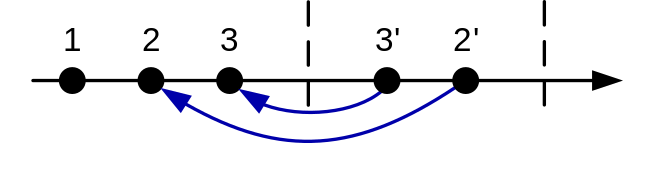
\includegraphics[width=0.8\textwidth]{../assets/kgeorgiy/transactions/Recovery_ARIES.svg.png}
	\caption{Иллюстрация компенсирующих записей при повторных сбоях}
	\label{recovery-aries}
\end{figure}

\begin{proposition}
	Компенсационные записи фиксируют прогресс восстановления БД и исключают повторный откат изменения
	при очередном восстановлении. Таким образом, повторные сбои не мешают завершению восстановления.
\end{proposition}

\subsubsection{Сравнение алгоритмов}

\paragraph{Число проходов}

\begin{itemize}
	\item \textbf{Классический алгоритм}. 3
	\item \textbf{Алгоритм ARIES}. 2
\end{itemize}

\paragraph{Рост журнала транзакций}

\begin{itemize}
	\item \textbf{Классический алгоритм}. В журнал добавляются записи отмены.
	\item \textbf{Алгоритм ARIES}. В журнал добавляются компенсирующие записи.
\end{itemize}

\paragraph{Повторные сбои}

\begin{itemize}
	\item \textbf{Классический алгоритм}. Полный перезапуск процесса восстановления.
	\item \textbf{Алгоритм ARIES}. Постепенное завершение.
\end{itemize}

\subsection{Транзакции. Параллельное исполнение. Блокировки.}

\subsubsection{Параллельное исполнение}

Напомним, что свойство \textit{изоляции (isolation)} транзакции подразумевает, что она должна исполняться
так, как будто она в системе одна, а также корректные по отдельности транзакции должны быть
корректными в совокупности. Следовательно, транзакции могут исполняться параллельно.

Обычно параллельные транзакции выполняются в разных потоках, что приводит к необходимости
использования блокировок для синхронизации.

\paragraph{Примеры конфликтов}

\begin{itemize}
	\item \textbf{Потерянное обновление (1)}. Обновление, сделанное транзакцией 1, потеряно.
	      \begin{center}
		      \begin{tabular}{|c c|}
			      \hline
			      Транзакция 1 & Транзакция 2 \\
			      \hline
			      retrieve T   &              \\
			                   & retrieve T   \\
			      update T     &              \\
			                   & update T     \\
			      commit       &              \\
			                   & commit       \\
			      \hline
		      \end{tabular}
	      \end{center}
	\item \textbf{Потерянное обновление (2)}. Обновление, сделанное транзакцией 1, потеряно.
	      \begin{center}
		      \begin{tabular}{|c c|}
			      \hline
			      Транзакция 1 & Транзакция 2 \\
			      \hline
			                   & update T     \\
			      update T     &              \\
			      commit       &              \\
			                   & rollback     \\
			      \hline
		      \end{tabular}
	      \end{center}
	\item \textbf{Незафиксированное изменение}. Значение, полученное транзакцией 1, не было
	      зафиксировано.
	      \begin{center}
		      \begin{tabular}{|c c|}
			      \hline
			      Транзакция 1 & Транзакция 2 \\
			      \hline
			                   & update T     \\
			      retrieve T   &              \\
			                   & rollback     \\
			      commit       &              \\
			      \hline
		      \end{tabular}
	      \end{center}
	\item \textbf{Несогласованное состояние}. Значение, полученное транзакцией 1, не могло быть
	      получено в согласованном состоянии.
	      \begin{center}
		      \begin{tabular}{|c c|}
			      \hline
			      Транзакция 1  & Транзакция 2            \\
			      \hline
			                    & update T\_1 = T\_1 - 10 \\
			      retrieve T\_1 &                         \\
			      retrieve T\_2 &                         \\
			                    & update T\_2 = T\_2 + 10 \\
			      commit        &                         \\
			                    & commit                  \\
			      \hline
		      \end{tabular}
	      \end{center}
\end{itemize}

\paragraph{Типы конфликтов}

\begin{itemize}
	\item \textbf{Чтение-чтение}. Нет конфликтов.
	\item \textbf{Чтение-запись}. Некорректное состояние.
	\item \textbf{Запись-чтение}. Зависимость от незафиксированного изменения.
	\item \textbf{Запись-запись}. Потерянное обновление.
\end{itemize}

\subsubsection{Блокировки}

Нам потребуются многоуровневые блокировки на фрагменты данных: разделяемая (для чтения,
\textit{S}) и эксклюзивная (для записи, \textit{X}). Отсутствие блокировки
обозначим \textit{-}.

\begin{definition}
	\textit{Протокол двухфазной блокировки}. Для чтения требуется получение \textit{S}, для
	записи -- \textit{X}, при завершении или откате транзакции требуется
	\textbf{последовательно} освободить все блокировки. Важно, что в первую фазу количество блокировок
	только растет, а во вторую -- только уменьшается.
\end{definition}

\begin{definition}
	\textit{Строгий протокол двухфазной блокировки}. Аналогично предыдущему определению,
	но все блокировки во второй фазе необходимо отпускать \textbf{после завершения или отката} транзакции.
\end{definition}

\paragraph{Взаимная блокировка (ВБ)}

\textbf{Пример взаимной блокировки}

\begin{center}
	\begin{tabular}{|c c|}
		\hline
		Транзакция 1  & Транзакция 2  \\
		\hline
		retrieve T\_1 &               \\
		              & retrieve T\_2 \\
		update T\_2   &               \\
		              & update T\_1   \\
		\hline
	\end{tabular}
\end{center}

Транзакция 1 и транзакция 2 сначала берут \textit{S} блокировки на чтение
\textit{T\_1} и \textit{T\_2} соответственно. Затем транзакция 1 пытается взять
\textit{X} блокировку на запись в \textit{T\_2}, что не удается сделать, пока
транзакция 2 владеет \textit{S} блокировкой \textit{T\_2}. Аналогично,
транзакция 2 не может взять \textit{X} блокировку на запись, поскольку так как
транзакция 1 владеет \textit{S} блокировкой на \textit{T\_2}.

\paragraph{Устранение ВБ}

\begin{itemize}
	\item \textbf{Построение графа ожиданий}. Наличие цикла в таком графе свидетельствует о ВБ. На
	      практике графы слишком большие, поэтому данный подход менее популярен.
	\item \textbf{Выставление таймаутов}. Отсутствие прогресса на протяжении долгого времени
	      вероятно свидетельствует о ВБ.
\end{itemize}

При обнаружении ВБ следует откатить одну из транзакций. Также, если СУБД владеет транзакцией, то
есть может ее перезапустить, то это следует сделать.

\paragraph{Предотвращение ВБ}

Пусть транзакция \textit{A} претендует на блокировку, конфликтующую с блокировками
транзакции \textit{B}. Возможны следующие стратегии.

\begin{itemize}
	\item \textbf{Стратегия ожидание-отмена}.
	      \begin{itemize}
		      \item \textit{A} началась раньше \textit{B} -- \textit{A} ожидает;
		      \item \textit{A} началась позже \textit{B} -- \textit{A} отменяется
		            (и, по
		            возможности, перезапускается);
	      \end{itemize}
	\item \textbf{Стратегия отмена-ожидание}.
	      \begin{itemize}
		      \item \textit{A} началась раньше \textit{B} -- \textit{B} отменяется
		            (и, по
		            возможности, перезапускается);
		      \item \textit{A} началась позже \textit{B} -- \textit{A} ожидает;
	      \end{itemize}
\end{itemize}

ВБ в каждой стратегии исключается, поскольку в графе ожидания ребра идут только от старшей к
младшей или от младшей к старшей транзакциям соответственно.

Стоит отметить, что стратегии порождают много лишних откатов.

\paragraph{Упорядочиваемость}

\begin{definition}
	\textit{Упорядочиваемость (serializability)} -- любая последовательность исполнения транзакций эквивалентна
	(равны состояния до начала и после окончания исполнения) некоторому последовательному
	исполнению.
\end{definition}

\begin{proposition}
	\textbf{Строгий} протокол двухфазной блокировки гарантирует упорядочиваемость.
\end{proposition}

\begin{proposition}
	Протокол двухфазной блокировки гарантирует упорядочиваемость.
\end{proposition}

\subsubsection{Восстановление и параллелизм}

Рассмотрим следующий пример.

\begin{center}
	\begin{tabular}{|c c|}
		\hline
		Транзакция 1 & Транзакция 2 \\
		\hline
		             & update T     \\
		retrieve T   &              \\
		commit       &              \\
		             & rollback     \\
		\hline
	\end{tabular}
\end{center}

Транзакция 1 фиксирует изменения, внесенные транзакцией 2. Однако, в будущем транзакция 2 может
быть откачена, например, из-за сбоя. Таким образом, фиксируется изменение, зависящее от
незафиксированного.

\begin{definition}
	\textit{Критерий восстанавливаемости}. Если транзакция \textit{A} использует значения,
	обновленные транзакцией \textit{B}, то \textit{A} должна завершиться позже,
	чем \textit{B}.
\end{definition}

В случае противоречий возникают взаимные блокировки, способы борьбы с которыми были рассмотрены
выше. Однако, это может привести к цепочкам форсированных откатов (откат транзакции
\textit{B} форсирует откат транзакции \textit{A}).

\begin{proposition}
	При строгом протоколе двухфазной блокировки цепочки отката отсутствуют.
\end{proposition}

\begin{proof}
	Транзакция \textit{A} сможет получить блокировку на чтение только после отпускания
	эксклюзивной блокировки на запись транзакцией \textit{B}. Последнее в строгом протоколе
	двухфазной блокировки произойдет только после завершения транзакции \textit{B}.
\end{proof}

\subsubsection{Гранулярность блокировок}

\begin{itemize}
	\item \textbf{Блокировка поля записи}. Блокируются отдельные поля каждой записи. Не
	      используется на практике.
	\item \textbf{Блокировка записей}. Блокируются отдельные записи. Дает высокий параллелизм и
	      требует больших ресурсов.
	\item \textbf{Блокировка страниц}. Блокируется страница памяти, на которой расположена запись.
	      Более практично по сравнению с блокировкой отдельных записей, поскольку на одной странице может
	      быть расположено много записей.
	\item \textbf{Блокировка индексов}. Блокируется элемент (например, поддерево в B-дереве или
	      корзина в хеш-индексе) или страница индекса. Запрещает добавление или удаление в рамках
	      заблокированного индекса.
	\item \textbf{Блокировка таблиц}. Блокируется таблица целиком. Требует мало ресурсов и
	      предоставляет низкий параллелизм.
	\item \textbf{Блокировка БД}. Используется для резервного копирования, изменения определения
	      таблиц и представлений, изменения хранимых процедур и функций и изменения прав доступа.
\end{itemize}

Аномалия \textbf{фантомные записи} -- при повторном чтении могут появиться новые записи. Возможна при
гранулярности блокировки меньше, чем по таблицам.

\subsection{Транзакции. Параллельное исполнение. Уровни изоляции.}

\paragraph{Уровни изоляции транзакций}

Мы рассматриваем следующие уровни изоляции транзакций. Все, кроме ``Слепок'', определены в
стандарте SQL.

\begin{itemize}
	\item \textbf{Упорядочиваемый (serializable)},
	\item \textbf{``Слепок'' (snapshot)},
	\item \textbf{Повторяемое чтение (repeatable read)},
	\item \textbf{Чтение зафиксированных (read committed)},
	\item \textbf{Чтение незафиксированных (read uncommitted)}.
\end{itemize}

\subsubsection{Упорядочиваемый}

Дает наиболее сильные гарантии с самой низкой скоростью исполнения. Детали реализации были
рассмотрены в предыдущем билете.

\subsubsection{``Слепок''}

Каждая транзакция работает со своим ``слепком'' БД. Вносит изменения в режиме copy-on-write. При
реинтеграции изменений они фиксируются, при отсутствии конфликтов изменений.

Является аналогом упорядочиваемого уровня изоляции с меньшими гарантиями, используется в
базах-``версионниках'', в которых синхронизация основана на версиях вместо блокировок.

\paragraph{Аномалия ``косая запись''}
На данном уровне изоляции возможна аномалия ``косая запись''. Она возникает при одновременном
обновлении разных записей, которые вместе должны гарантировать некоторый инвариант.

\textbf{Пример}. Положим инвариант $\texttt{t\_1} + \texttt{t\_2} \geq 0$.

\begin{itemize}
	\item Транзакция 1
	      \begin{lstlisting}[language=SQL]
            if t_1 + t_2 >= DELTA begin
                t_1 = t_1 - DELTA
            end if
        \end{lstlisting}
	\item Транзакция 2
	      \begin{lstlisting}[language=SQL]
            if t_1 + t_2 >= DELTA begin
                t_2 = t_2 - DELTA
            end if
    \end{lstlisting}
\end{itemize}

Реинтеграция изменений пройдет успешно, поскольку записи идут в разные переменные. Однако, при
параллельном исполнении инвариант может быть нарушен.

\subsubsection{Повторяемое чтение}

Уровень изоляции гарантирует, что при повторном чтении значения не будут меняться. Исключение --
запись, произведенная самой транзакцией. Реализуется путем взятия блокировок записей или страниц на
чтение.

\paragraph{Аномалия ``фантомная запись''}

При повторном чтении могут появиться новые записи. Возможно при параллельном исполнении другой
транзакции.

\subsubsection{Чтение зафиксированных}

Уровень изоляции гарантирует, что читаемые значения зафиксированы другими транзакциями. Реализуется
путем взятия \textit{частичных} блокировок записей или страниц на чтение.

\paragraph{Аномалия ``неповторяемое чтение''}

При повторном чтении могут значение записи может измениться. Возможно при параллельном исполнении
другой транзакции.

\subsubsection{Чтение незафиксированных}

На уровне изоляции не используются блокировки, что обеспечивает наивысшую скорость. По стандарту
SQL разрешено только чтение. Используется для сбора статистики.

\paragraph{Аномалия ``грязное чтение''}

Может быть прочитано некорректное значение.

\subsection{Оптимизация запросов. Выбор методов исполнения запроса}

\begin{definition}
	\textit{Сеть операций} -- граф вычислений запросов в реляционной алгебре. Аргументы для каждого
	узла -- базовые таблицы или результаты других операций, результат узла является либо аргументом
	другого узла.
\end{definition}

В графе выделяют два типа  узлов:

\begin{itemize}
	\item \textbf{Преобразователи} -- просматривают аргументы в процессе работы и не хранят
	      информацию в памяти. Другими словами, из таких операций записи можно получать по одной записи.
	      Используют внутри себя курсоры.
	\item \textbf{Контейнеры} -- загружают аргументы, сохраняют результаты, при необходимости -- на
	      диске. В отличие от преобразователей требуют все входные данные вместе для выполнения операции.
\end{itemize}

Пример сети операций приведен на рисунке \ref{operation-network}. Синим цветом отмечены
преобразователи, зеленым -- контейнеры.

\begin{figure}[H]
	\centering
	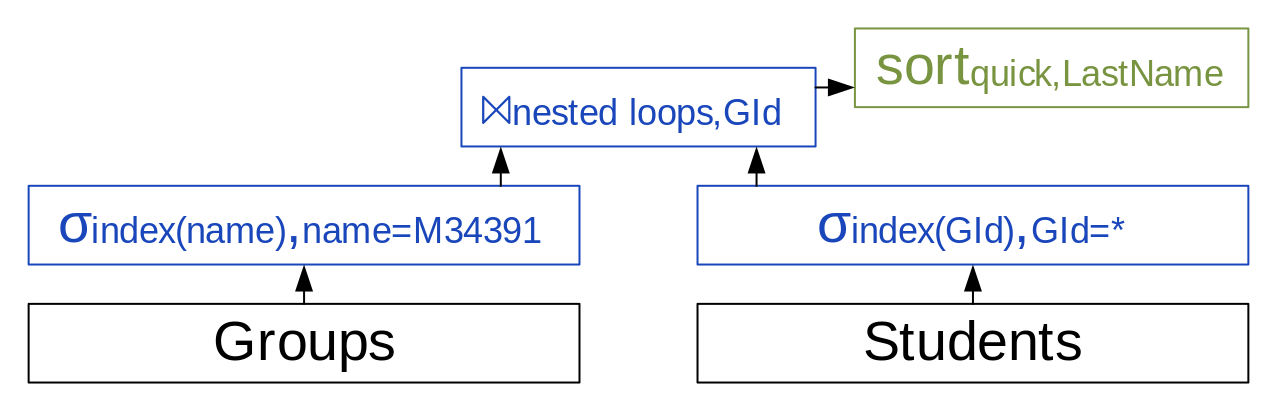
\includegraphics[width=0.8\textwidth]{../assets/kgeorgiy/optimization/Network_Students_Types.svg.png}
	\caption{Пример сети операций}
	\label{operation-network}
\end{figure}

\paragraph{Унарные операции}

\begin{itemize}
	\item \textbf{Фильтрация}. Преобразователь. игнорирует строки, не удовлетворяющие условию.
	      \begin{itemize}
		      \item \textit{Трудоемкость}: $\mathcal{O}(n)$, где $n$ -- размер входных данных;
		      \item \textit{Свойства}: Операция может существенно уменьшать количество обрабатываемых
		            строк, что учитывается в планировщике путем оценки селективности.
	      \end{itemize}
	\item \textbf{Проекция}. Преобразователь. В случае, если указан \texttt{distinct}, удаляет
	      дубликаты по проецируемым атрибутам, иначе только помечает, какие атрибуты больше не требуются.
	      \begin{itemize}
		      \item \textit{Трудоемкость}: $\mathcal{O}(n)$, где $n$ -- размер входных данных;
		      \item \textit{Свойства}: данные на входе должны быть упорядочены, результат операции
		            сохраняет порядок.
	      \end{itemize}
	\item \textbf{Сортировка}. Контейнер. Если данные помещаются в оперативную память, производится
	      сортировку в ней, иначе применяется внешняя сортировка, которая значительно менее производительна.
	      \begin{itemize}
		      \item \textit{Трудоемкость}: $\mathcal{O}(n \log(n))$, где $n$ -- размер входных данных;
		      \item \textit{Свойства}: результат операции -- упорядоченные данные, время исполнения
		            скачкообразно зависит от объема входных данных (скачок происходит при аллокации новой памяти).
	      \end{itemize}
	\item \textbf{Просмотр таблиц}. В зависимости от реализации -- преобразователь (полный проход
	      по таблице) или контейнер (выдача в отсортированном виде).
	      \begin{itemize}
		      \item \textit{Трудоемкость}: $\mathcal{O}(n)$, где $n$ -- размер входных данных;
		      \item \textit{Методы исполнения}: полный просмотр, использование индекса,
		            использование кластеризованного индекса.
	      \end{itemize}
\end{itemize}

\paragraph{Множественные операции}

\begin{itemize}
	\item \textbf{Объединение}. Преобразователь. Производит слияние двух аргументов.
	      \begin{itemize}
		      \item \textit{Трудоемкость}: $\mathcal{O}(n)$, где $n$ -- размер входных данных;
		      \item \textit{Свойства}: ожидается, что аргументы упорядочены, результат также будет
		            упорядочен.
	      \end{itemize}
	\item \textbf{Пересечение}. Полностью аналогично объединению.
	\item \textbf{Разность}. Полностью аналогично объединению.
\end{itemize}

\paragraph{Соединения}

Существует несколько подходов построения соединений.

\begin{itemize}
	\item \textbf{Вложенный перебор}. Преобразователь. Для каждой строки левого аргумента ищет
	      строку из правого аргумента полным перебором.
	      \begin{itemize}
		      \item \textit{Трудоемкость}: $\mathcal{O}(l \cdot r)$, где $l$, $r$
		            -- размеры левого и
		            правого аргументов;
		      \item \textit{Свойства}: сохраняет упорядоченность (по столбцам левого аргумента, при
		            равенстве левого аргумента -- по столбцам правого).
	      \end{itemize}
	\item \textbf{Поиск по дереву}. Преобразователь. Для каждой строки левого аргумента ищет
	      строку из правого аргумента с помощью индекса. Применим если уже построен индекс методом дерева.
	      \begin{itemize}
		      \item \textit{Трудоемкость}: $\mathcal{O}(\max(l \cdot \log(r), n))$, где $l$, $r$
		            --
		            размеры левого и правого аргументов, $n$ -- размер выхода;
		      \item \textit{Свойства}: сохраняет упорядоченность (аналогично вложенному перебору).
	      \end{itemize}
	\item \textbf{Поиск по хешу}. Преобразователь и контейнер. Перед соединением правый аргумент
	      хешируется. Для каждой строки левого аргумента ищет строку из правого аргумента с помощью хеша.
	      Если хеш-индекс уже построен, может переиспользовать его.
	      \begin{itemize}
		      \item \textit{Трудоемкость}: $\mathcal{O}(\max(l + r, n))$, где $l$, $r$
		            --
		            размеры левого и правого аргументов, $n$ -- размер выхода.
	      \end{itemize}
	\item \textbf{Слияние}. Преобразователь. Применим если входные аргументы упорядочены по общим
	      атрибутам. Производится стандартным алгоритмом слияния.
	      \begin{itemize}
		      \item \textit{Трудоемкость}: $\mathcal{O}(\max(l + r, n))$, где $l$, $r$
		            --
		            размеры левого и правого аргументов, $n$ -- размер выхода;
		      \item \textit{Свойства}: требует упорядоченности аргументов, сохраняет упорядоченность.
	      \end{itemize}
\end{itemize}

\subsection{Секционирование}

\begin{definition}
	\textit{Секционирование} -- разбиение таблицы на фрагменты, хранящиеся в разных местах (в
	случае разных компьютеров называется \textit{шардинг}). Используется для увеличения скорости
	чтения за счет параллельного обращения.
\end{definition}

Различают два вида секционирования: \textbf{вертикальное} и \textbf{горизонтальное}.

\subsubsection{Вертикальное секционирование}

Таблица разбивается по столбцам. Возможно при корректности соединения (5 НФ). Реализуется
посредством проекции и соединения.

\paragraph{Преимущества}

\begin{itemize}
	\item Отделение данных, к которым часто обращаются, от тех, к которым обращаются редко.
	\item Защита информации.
	\item Поддерживается во многих СУБД для \texttt{CLOB} и \texttt{BLOB}.
\end{itemize}

\paragraph{Недостатки}

\begin{itemize}
	\item Нет специальной поддержки в СУБД. Считается, что проекции и соединения для указанных целей
	      достаточно.
	\item Зависимость от представления (соединенных данных). Некоторые СУБД накладывают ограничения на
	      представления, например, запрещают создавать внешние ключи на них.
	\item Необходимость обновляемых представлений также не гарантирована.
\end{itemize}

\paragraph{Пример}

Рассмотрим исходную таблицу.

\begin{lstlisting}
    Students(SId, GId, FirstName, LastName, PassSeries,
        PassNo, PassIssued, Photo)
\end{lstlisting}

Разобьем ее на секции.

\begin{lstlisting}
    StudentData(SId, GId, FirstName, LastName)
    StudentPasses(SId, PassSeries, PassNo, PassIssued)
    StudentPhotos(SId, Photo)
\end{lstlisting}

Обращение к фото (\texttt{StudentPhotos}) происходит значительно реже, чем к основным данным
студента (\texttt{StudentData}). Также таблица с персональными данными (\texttt{StudentPasses})
требует повышенных прав доступа. Таким образом, были использованы все преимущества вертикального
секционирования.

Создадим также представление для работы с исходной таблицей.

\begin{lstlisting}[language=SQL]
    create view Students as StudentData
        natural join StudentPasses
        natural join StudentPhotos;
\end{lstlisting}

\subsubsection{Горизонтальное секционирование}

Таблица разделяется по строкам. Корректно, когда каждая строка попадает ровно в одну секцию.
Реализуется посредством фильтрации и объединения.

\paragraph{Преимущества}

\begin{itemize}
	\item Отделение данных, к которым часто обращаются, от тех, к которым обращаются редко. Например, чаще
	      всего старые данные нужны реже новых.
	\item При уменьшении размера секции уменьшается размер индекса.
	\item Требуется встроенная поддержка.
	\item Прозрачно для пользователя.
\end{itemize}

\paragraph{Недостатки}

\begin{itemize}
	\item В некоторых случаях может приводить к замедлению работы.
\end{itemize}

\paragraph{Пример}

Рассмотрим исходную таблицу.

\begin{lstlisting}
    Points(SId, CId, Points, Date)
\end{lstlisting}

Введем секционирование по Date:

\begin{itemize}
	\item $\texttt{Points}_{2021-1}$ -- оценки за весенний семестр 2021,
	\item $\texttt{Points}_{2021-2}$ -- оценки за осенний семестр 2021,
	\item $\texttt{Points}_{2020-1}$ -- оценки за весенний семестр 2020,
	\item \ldots
\end{itemize}

\paragraph{Методы секционирования}

\begin{itemize}
	\item \textbf{Простые}.
	      \begin{itemize}
		      \item По диапазонам значений,
		      \item По значениям,
		      \item По хешу.
	      \end{itemize}
	\item \textbf{По выражению}. Поддерживаются реже.
	\item \textbf{Составные}.
	      \begin{itemize}
		      \item По диапазонам и хешу,
		      \item \ldots
	      \end{itemize}
\end{itemize}

\paragraph{Пример} Секционирование по диапазонам.

\begin{lstlisting}[language=SQL]
    create table Points(...)
    partition by range(Date) (
        partition pHist values less than '2021-02-01',
        partition p2021s1 values less than '2021-07-01',
        partition p2021s2 values less than '2022-02-01',
        partition pFuture values less than maxvalue
    );
\end{lstlisting}

\texttt{maxvalue} -- максимальное теоретическое значение.

\paragraph{Пример} Секционирование по значениям.

Чаще используется для перечислений.

\begin{lstlisting}[language=SQL]
    create table Points(...)
    partition by list(Term) (
        partition pHist values in ('t2020-1', 't2020-2', ...),
        partition p2021s1 values in ('t2021-1'),
        partition p2021s2 values in ('t2021-2'),
        partition pFuture values in ('t2022-1')
    );
\end{lstlisting}

При таком подходе секция может быть не определена при записи.

\begin{lstlisting}[language=SQL]
    insert into Points (Term) values ('t2001-1');
\end{lstlisting}

При чтении из несуществующей секции будет получен пустой результат.

\paragraph{Пример} Секционирование по хешу.

Хешируется по набору столбцов. Работает эффективно при хорошей и быстрой хеш-функции.

\begin{lstlisting}[language=SQL]
    create table Points(...)
    partition by hash(Term)
    partitions 4;
\end{lstlisting}

\paragraph{Пример} Секционирование по выражению.

Зависит от определенной в БД функции.

\begin{lstlisting}[language=SQL]
    create table Points(...)
    partition by year(Date) (
        partition pHist values less than 2021,
        partition pCurrent values less than 2022,
        partition pFuture values less than maxvalue
    );
\end{lstlisting}

\paragraph{Пример} Составное секционирование.

Секции разбиваются на подсекции, возможно, по разным атрибутам.

\begin{lstlisting}[language=SQL]
    create table Points(...)
    partition by year(Date)
    subpartition by hash(Term) (
        partition History values less than 2021 (
            subpartition History1, subpartition History2
        ),
        partition Current values less than 2022 (
            subpartition Current1, subpartition Current2
        )
    );
\end{lstlisting}

\paragraph{Управление секциями}

\begin{remark}
	Данные команды не входят в стандарт SQL, поэтому синтаксис может отличаться в зависимости от СУБД.
\end{remark}

\textbf{Удаление секции}

\begin{lstlisting}[language=SQL]
    alter table <table> drop partition <section>;
\end{lstlisting}

\textbf{Разбиение секции}

\begin{lstlisting}[language=SQL]
    alter table <table> reorganize <section> into (...);
\end{lstlisting}

\textbf{Перехеширование}

\begin{lstlisting}[language=SQL]
    -- Добавить число разделов
    alter table <table> add partition <count>;
    -- Удалить число разделов
    alter table <table> coalesce partition <count>;
\end{lstlisting}

\begin{proposition}
	Оптимизатор владеет информацией о секциях. В частности, где какие данные находятся.
\end{proposition}

\paragraph{Пример}

\begin{lstlisting}[language=SQL]
    select * from Points where Date = '2021-12-06
\end{lstlisting}

При таком запросе выборка будет производиться только из секции 2021 года.

\paragraph{Секционирование и индексы}

Можно определить следующие индексы:

\begin{itemize}
	\item \textbf{Локальный} -- один на секцию. Ускорение при выборе секций.
	\item \textbf{Глобальный} -- один на таблицу. Также ускорение при выборе секций.
	\item \textbf{Секционированный} -- разбит на секции. Обеспечивает согласованное
	      секционирование (могут помочь при склеивании секций).
\end{itemize}

\paragraph{Секционирование и ключи}

Лучше всего, если множество столбцов, по которым идет секционирование, образует подключ. Еще лучше
-- подключ всех ключей (например, если внешние ключи на таблицу ссылаются на разные ее ключи).

\subsection{Репликация}

\begin{definition}
	\textit{Репликация} -- поддержание одинаковых данных на нескольких узлах.
\end{definition}

\subsubsection{Реализация репликации}

Репликация бывает \textbf{синхронной} (с использованием распределенных транзакций) и \textbf{асинхронной} (информация до реплик доходит с задержками). С другой стороны, различают
схемы репликации \textbf{c основной копией} и \textbf{симметричную}.

\paragraph{Репликация с основной копией}

\begin{figure}[h]
	\centering
	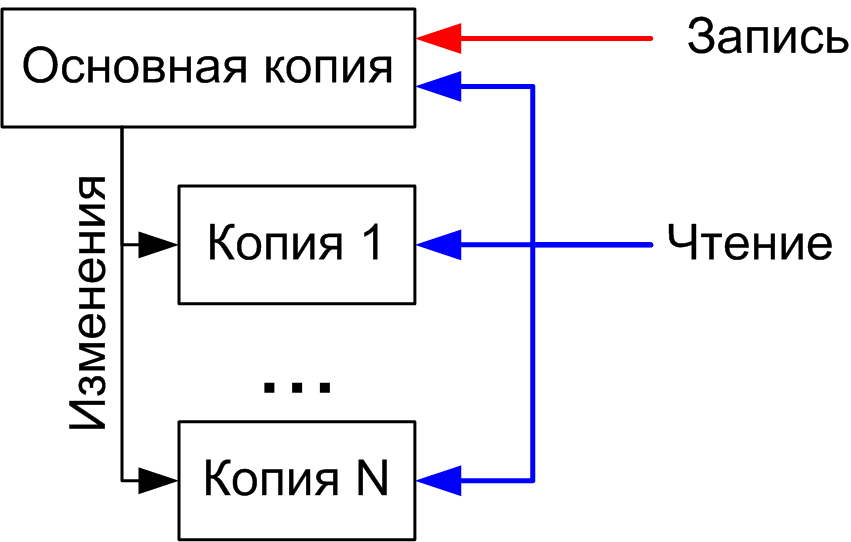
\includegraphics[width=0.8\textwidth]{../assets/kgeorgiy/distributed/Replication_Master.png}
	\caption{Схема репликации с основной копией}
	\label{repl-master}
\end{figure}

Чтение данных можно производить из любой копии БД, в то время как запись -- только в основную.
Согласованность всех копий обеспечивается за счет проверки при записи в основную копию. Данная
схема подходит, если число записей сильно меньше числа чтений.

\paragraph{Симметричная репликация}

\begin{figure}[h]
	\centering
	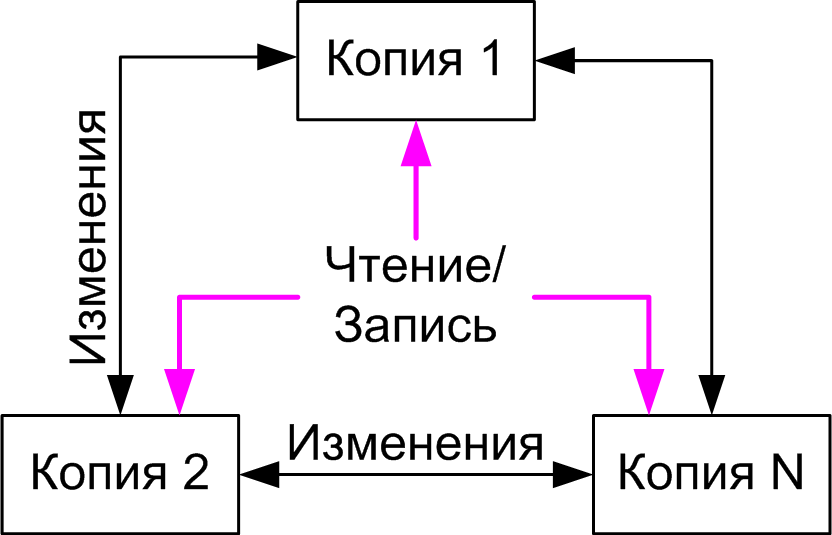
\includegraphics[width=0.8\textwidth]{../assets/kgeorgiy/distributed/Replication_Symmetric.png}
	\caption{Схема симметричной репликации}
	\label{repl-symm}
\end{figure}

Чтение и запись производятся в каждую копию независимо, все копии равноправны и автономны. Для
борьбы с противоречивыми изменениями в данной схеме требуется синхронность изменений.

\paragraph{Реализация репликации}

Данные об изменениях можно рассылать из журнала транзакций. Можно рассылать данный в различной
гранулярности:

\begin{itemize}
	\item \textbf{Репликация операторов}. При таком подходе используется меньше данных. Однако,
	      каждый оператор должен быть детерминированным, а также необходимо учитывать взаимный порядок
	      выполнения транзакций. Сложно для реализации.
	\item \textbf{Репликация записей}. Рассылается информация об изменении отдельных записей. При
	      таком подходе нет требования к детерминированности. Однако, крупные обновления данных приведут к
	      рассылке больших сообщений.
\end{itemize}

\subsubsection{Применения репликации}

\paragraph{Вертикальное масштабирование}

При необходимости вертикального масштабирования (наращивания мощности системы) следует использовать
\textbf{асимметричную схему}. Напомним, что ее использование целесообразно, когда количество изменений
гораздо меньше количества чтений.

Применяется в ситуациях, когда допустима асинхронность. Например, в Web-серверах и ERP-системах.

\paragraph{Горизонтальное масштабирование}

В ситуациях, когда необходимо производить множество локальных операций, например, в разных
географических областях, применяется \textbf{симметричная схема}. Каждая реплика отвечает за
определенные данные в зависимости от запроса. Также этот подход полезен в случае непостоянной
связи.

\paragraph{Повышение доступности}

Для повышения доступности данных следует использовать \textbf{асимметричную схему}, которая позволяет
менять основную реплику при выходе из строя прошлой. В случае синхронной репликации потери данных
отсутствуют, однако, в случае асинхронной вышедшая из строя основная реплика могла не успеть
разослать другим репликам изменения.

Также полезно \textbf{резервное копирование} БД. В асимметричной схеме для этого достаточно создать
реплику, с которой постоянно синхронизируется основная. Для создания резервной копии достаточно
отключить такую реплику, скопировать данные, включить обратно в систему и восполнить пропущенные
обновления.

\paragraph{Преобразование данных}

Используется \textbf{асимметричная схема}, которая предоставляет отлаженный способ получения всех
изменений данных. На основе них можно строить преобразование данных: изменение формата хранения,
консолидация, унификация, подсчет статистики и так далее. Таким образом, преобразования происходят
при репликации.
\subsection{Распределенные транзакции}

\begin{definition}
	\textit{Распределенные транзакции} -- транзакции, в которых участвует несколько узлов. Каждая
	транзакция должна быть либо применена, либо откачена на всех узлах одновременно.
\end{definition}

В рамках распределенных транзакций необходимо рассматривать сбои как \textit{участников}, так и
\textit{коммуникаций}.

\paragraph{Протокол двухфазной транзакции}

Классический подход реализации распределенных транзакций. Один из узлов выбирается координатором
(как правило, узел, на который пришел запрос). Это означает, что при параллельном исполнении
нескольких транзакций несколько узлов одновременно могут быть координаторами.

Далее каждая транзакция проходит через две фазы.

\begin{figure}[h]
	\centering
	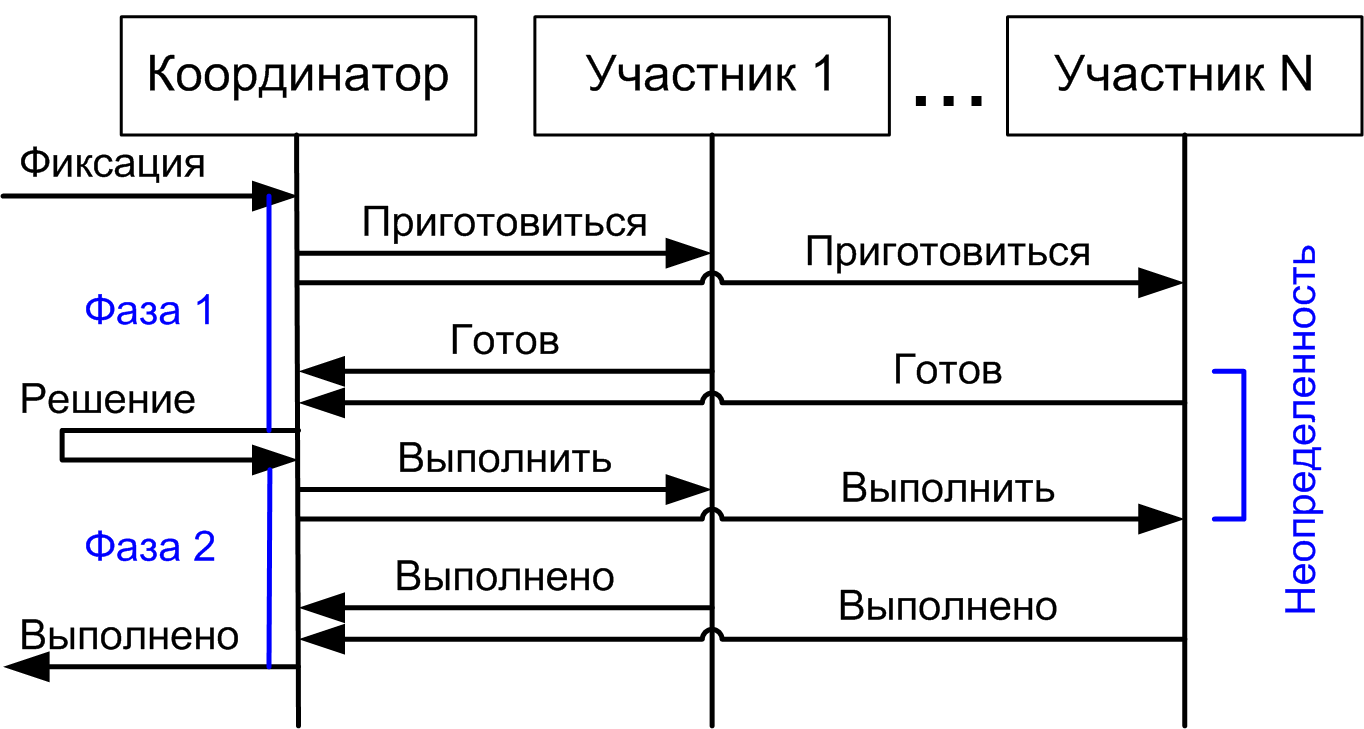
\includegraphics[width=0.8\textwidth]{../assets/kgeorgiy/distributed/Distributed_TwoPhase.png}
	\caption{Схема протокола двухфазной транзакции}
	\label{2-phase-tx}
\end{figure}

\begin{itemize}
	\item \textbf{Фаза подготовки}. Координатор рассылает информацию об изменении всем другим
	      копиям. Далее эти копии должны ответить, что готовы зафиксировать изменение (нет противоречий,
	      данные находятся в согласованном состоянии, нет иных ошибок).
	\item \textbf{Решение координатора}. После получения ответов от всех копий, координатор
	      принимает решение, выполнять ли фиксацию данных. Решение положительное, если от все пришедшие
	      ответы от других копий положительные.
	\item \textbf{Фаза выполнения}. При положительном решении координатор рассылает сообщение о
	      том, что изменения должны быть зафиксированы, и ожидает подтверждения этого от всех копий.
	\item \textbf{Результат}. Если координатор получает подтверждения от всех копий, то транзакция
	      считается выполненной.
\end{itemize}

Если \textit{координатор} не получил хотя бы одно подтверждение на первой фазе, то транзакция
автоматически откатывается. Как только принимается решение о фиксации, оно записывается в журнал
транзакций координатора -- так копии смогут заново воспроизвести решение при восстановлении.
Однако, если координатор не получил хотя бы одно подтверждение на второй фазе, то это неразрешимая
ситуация.

\textit{Копии} при сбое до отправки подтверждения на первой фазе должны откатить
транзакцию, поскольку координатор не мог принять решения о фиксации без подтверждения. При сбое до
получения решения о фиксации копия должна запросить решение снова у координатора. При получении
решения о фиксации копия записывает в свой журнал транзакций изменение для восстановления в
будущем.

Однако, задача теоретически не разрешима. То есть существует сценарий, при котором ни координатор,
ни реплика не смогут продвинуться (но эти случаи вырождены). Это показывает отсутствие решения
следующей задачи.

\paragraph{Задача двух генералов}

Генералам двух армий необходимо напасть на врага. Они достигнут успеха только если нападут
одновременно. Им необходимо прийти к \textit{консенсусу}: нападать или нет. Генералы могут
посылать гонцов с сообщениями, которых могут убить в пути.

\begin{proposition}
	Не существует гарантированного решения задачи двух генералов.
\end{proposition}

\begin{proof}
	Предположим противное: существует конечный протокол, при использовании которого можно прийти к
	консенсусу. Следовательно, существует минимальное по включению множество сообщений, которые
	необходимо отправить. Предположим, что последнее сообщение не было доставлено. Тогда невозможно
	принять решение. Противоречие.
\end{proof}

\paragraph{Протоколы предполагаемой фиксации и отката}

Как было показано выше, копии могут запрашивать решение у координатора повторно. Таким образом,
координатору необходимо сохранить информацию о решении до тех пор, пока не получит подтверждения от
всех копий. Рассмотрим два подхода оптимизации объема памяти, занимаемого решениями координатора.

\begin{itemize}
	\item \textbf{Протокол предполагаемой фиксации}. При решении о фиксации транзакции она
	      ``забывается'' координатором. Если координатор получает запрос о решении по неизвестной ему
	      транзакции, то он отвечает, что ее нужно зафиксировать. Данный подход позволяет сэкономить память,
	      если число зафиксированных транзакций сильно превышает число откаченных.
	\item \textbf{Протокол предполагаемого отката}. При решении об откате транзакции она
	      ``забывается'' координатором. Если координатор получает запрос о решении по неизвестной ему
	      транзакции, то он отвечает, что ее нужно откатить. Данный подход позволяет сэкономить память, если
	      число откаченных транзакций сильно превышает число зафиксированных.
\end{itemize}

\begin{remark}
	Протокол предполагаемой фиксации может привести к ложной фиксации. Например, если информация о
	решении была ошибочно утеряна. В таком случае всем другим участникам будет приходить ответ о
	фиксации, которой в действительности не было. Поэтому рекомендуется использовать протокол
	предполагаемого отката.
\end{remark}

\subsection{Распределенные базы данных. Цели и проблемы}

\subsubsection{Цели распределения}

Определим ряд целей, которые стремятся достигнуть при разработке распределенных баз данных.

\begin{itemize}
	\item \textbf{Децентрализация}.
	      \begin{itemize}
		      \item \textit{Локальная независимость}. Узел должен продолжать функционировать даже в
		            изоляции от других.
		      \item \textit{Отсутствие центрального узла}. При наличии такового отказ этого узла
		            приведет к отказу системы целиком, что есть уязвимость.
		      \item \textit{Непрерывное функционирование}. Хранилище данных должно быть надежным и
		            доступным.
	      \end{itemize}
	\item \textbf{Прозрачность}.
	      \begin{itemize}
		      \item \textit{Независимость от расположения}. Логически программы должны работать на
		            произвольном узле и обеспечивать удаленный доступ к данным. Иными словами, распределенная БД с
		            точки зрения пользователя должна себя вести так же, как если бы она представляла собой одну
		            большую. При этом нет требований к временным задержкам.
		      \item \textit{Независимость от фрагментации}. Программы не должны зависеть от
		            информации об узле, на котором находятся данные. Доступ должен быть унифицированным.
		      \item \textit{Независимость от репликации}. Должна быть поддержана автоматически.
	      \end{itemize}
	\item \textbf{Распределенные транзакции}.
	      \begin{itemize}
		      \item \textit{Поддержка распределенных запросов}. Получение данных с разных узлов в
		            рамках одного запроса.
		      \item \textit{Поддержка распределенных записей}. Несколько узлов должны участвовать в
		            единой транзакции. При этом необходима согласованность фиксации и отката.
	      \end{itemize}
	\item \textbf{Независимость от окружения}.
	      \begin{itemize}
		      \item \textit{Независимость от аппаратуры}. Унифицированное представление данных.
		      \item \textit{Независимость от ОС}. Прозрачная поддержка различных ОС и конвертация
		            данных. Один узел может быть запущен на Windows, а другой -- на Ubuntu.
		      \item \textit{Независимость от сети}. Прозрачная поддержка различных сетей. Копии могут
		            быть как расположены внутри одного датацентра, так и разнесены географически.
		      \item \textit{Независимость от типа СУБД}. Прозрачная поддержка различных СУБД и
		            конвертация данных.
	      \end{itemize}
\end{itemize}

Из требований децентрализации следует равноправие узлов, что влечет за собой решение задач
распределенного консенсуса, в частности, выбора лидера.

\begin{remark}
	Важно, что распределенные базы данных отличаются от репликации тем, что каждый узел реально владеет
	данными, расположенными на нем. То есть каждая запись лежит ровно на одном узле.
\end{remark}

\subsubsection{Проблемы распределения}

\begin{theorem}[CAP-теорема]
	Одна система может обладать не более чем двумя свойствами из нижеуказанных
	одновременно:
	\begin{itemize}
		\item \textit{Consistency (C)} -- информация на разных узлах согласована;
		\item \textit{Availability (A)} -- система отвечает на запросы в любой момент времени;
		\item \textit{Partition tolerance (P)} -- система работает корректно при обрыве связи между узлами.
	\end{itemize}
\end{theorem}

\begin{remark}
	Важно, что вышеуказанные свойства не бинарны, в то время как доказательство теоремы верно только
	для бинарных свойств. Например, если допускается, что согласованность может периодически
	нарушаться, то применение теоремы некорректно, и такую систему теоретически можно реализовать.
	Таким образом, систему со всеми свойствами реализовать возможно, но частично уступив в некоторых
	свойствах.
\end{remark}

Обычно теорему рассматривают с точки зрения свойства \textit{P}, поскольку при
отсутствии \textit{P} система не разделена.

\begin{itemize}
	\item Система реализуема при частичном отказе от \textit{A}. Следовательно, при обрыве связи
	      в системе функционирует только одна ее часть.
	\item Система реализуема при частичном отказе от \textit{C}. Следовательно, системе необходим
	      механизм объединения состояний.
\end{itemize}

Поскольку свойства CAP-теоремы слишком сильные для одновременной поддержки, рассматривают подход с
ослабленными свойствами.

\begin{definition}
	\textit{Свойства BASE}.
	\begin{itemize}
		\item \textit{Basically Available (BA)} -- сбой узла приводит к отказу только для части
		      пользователей;
		\item \textit{Soft-state (S)} -- изменения в системе могут происходить не только по причине
		      внешнего вмешательства (например, при восстановлении соединения);
		\item \textit{Eventual consistency (E)} -- несогласованность устраняется со временем.
	\end{itemize}
\end{definition}

\paragraph{Восстановлени согласованности}

При восстановлении согласованности можно использовать следующие подходы: при чтении, при записи или
асинхронно. Первые два варианта замедляют соответствующие операции, асинхронный подход требует
создания специального процесса. Для разрешения используются механизмы меток времени и векторные
часы.

\paragraph{Оптимизация запросов}

В распределенной системе задача оптимизации запросов дополнительно усложняется. Дополнительно
необходимо минимизировать количество доступов к удаленным данным.

Добиться этого можно следующими средствами:

\begin{itemize}
	\item \textbf{Выбор узлов получения и обработки данных}. Например, лучше выполнять запрос на
	      узле, который владеет большей долей затрагиваемых данных локально для минимизации коммуникаций.
	\item \textbf{Полусоединения}. Позволяют запрашивать с других узлов только необходимые данные.
	\item \textbf{Применение репликации}. Для получения данных может быть достаточным обращение к
	      реплике.
\end{itemize}

\paragraph{Управление параллельностью}

Базы данных, основанные на блокировках, требуют реализации механизмов распределенных блокировок и
детектирования распределенных взаимных блокировок. Это усложняет параллелизацию запроса и изоляцию
транзакций. Основные средства для решения: использование более сложлных распределенных алгоритмов и
схемы с основной копией.

\paragraph{Управление каталогом}

Каталог также может быть распределен. Однако, традиционно используются СУБД, в которых считается,
что каталог один. Информация о каталоге полностью реплицируется на все узлы.

\paragraph{Независимость от окружения}

\begin{figure}[h]
	\centering
	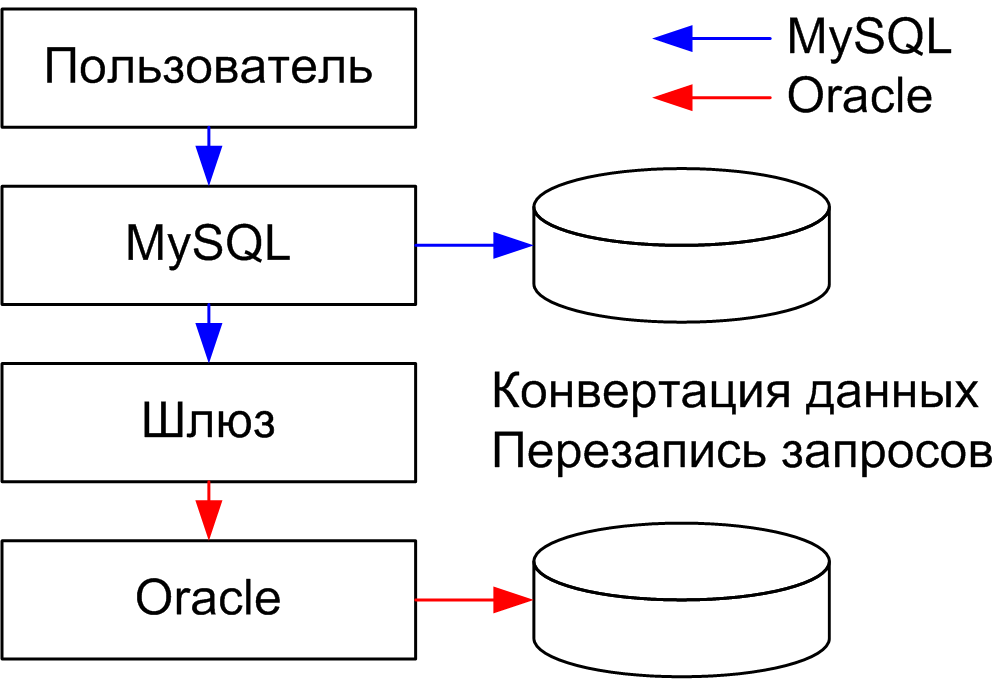
\includegraphics[width=0.8\textwidth]{../assets/kgeorgiy/distributed/Distributed_Gateway.png}
	\caption{Схема обеспечения прозрачности при использовании различных СУБД}
	\label{env-independence}
\end{figure}

Для обеспечения независимости от реализации СУБД используется механизм шлюзов, которые решают
задачи конвертации данных и перезаписи запросов. Например, Oracle предоставляет шлюз с MySQL.

Со стороны шлюх выглядит как очередная сущность СУБД. Также ожидается, что он поддерживает
распределенные транзакции и блокировки.

\subsection{Трактовки null и операции с ним}

\subsubsection{Трактовки null}

SQL допускает использования в качестве значения \texttt{null} по умолчанию. Однако, это
значение может трактоваться по-разному.

Рассмотрим для этого следующий пример: пусть в БД ``Университет'' идентификатор группы студента
равен \texttt{null}, то есть значение отсутствует. Это может означать одно следующего:

\begin{itemize}
	\item \textbf{Значение не известно}. Неизвестно, в какой группе обучается студент;
	\item \textbf{Значение не верно}. Студент учится в группе, имя которой неверно;
	\item \textbf{Значение еще не существует}. Студент зачислен, но не определен в группу;
	\item \textbf{Значение уже не существует}. Группа отчисленного студента;
	\item \textbf{Значение не имеет смысла}. Студент из другого университета;
	\item \textbf{Значение не доступно}. У пользователя нет права узнать группу.
\end{itemize}

Заметим, что отсутствующие значения можно реализовать без \texttt{null} -- используя
необязательную связь 1:1. Однако, \texttt{null} может появиться в результате
множественных операций и внешних соединений. Поэтому полностью \texttt{null} исключить
нельзя.

\subsubsection{Операции с null}

\paragraph{Тернарная логика}

С точки зрения SQL \textit{результат} результат логического выражения может быть
\texttt{true}, \texttt{false} или \texttt{unknown}. Однако, тип
\texttt{boolean} может \textit{принимать значения} \texttt{true},
\texttt{false} или \texttt{null}. С практической точки зрения,
\texttt{unknown} и \texttt{null} не отличаются.

Рассмотрим основные логические опреации.

\begin{center}
	\begin{tabular}{|c||c|c|c|}
		\hline
		\textbf{AND}     & \texttt{true}    & \texttt{unknown} & \texttt{false} \\
		\hline
		\hline
		\texttt{true}    & \texttt{true}    & \texttt{unknown} & \texttt{false} \\
		\hline
		\texttt{unknown} & \texttt{unknown} & \texttt{unknown} & \texttt{false} \\
		\hline
		\texttt{false}   & \texttt{false}   & \texttt{false}   & \texttt{false} \\
		\hline
	\end{tabular}
\end{center}

\begin{center}
	\begin{tabular}{|c||c|c|c|}
		\hline
		\textbf{OR}      & \texttt{true} & \texttt{unknown} & \texttt{false}   \\
		\hline
		\hline
		\texttt{true}    & \texttt{true} & \texttt{true}    & \texttt{true}    \\
		\hline
		\texttt{unknown} & \texttt{true} & \texttt{unknown} & \texttt{unknown} \\
		\hline
		\texttt{false}   & \texttt{true} & \texttt{unknown} & \texttt{false}   \\
		\hline
	\end{tabular}
\end{center}

\begin{center}
	\begin{tabular}{|c||c|c|c|}
		\hline
		\textbf{NOT} & \texttt{true}  & \texttt{unknown} & \texttt{false} \\
		\hline
		\hline
		             & \texttt{false} & \texttt{unknown} & \texttt{true}  \\
		\hline
	\end{tabular}
\end{center}

Интуитивно, \texttt{true} > \texttt{unknown} > \texttt{false}.
\textbf{AND} возвращает меньшее из аргументов, \textbf{OR} -- большее из
аргументов, \textbf{NOT} -- обратное по порядку.

Для сравнения используются два оператора: бинарный \textbf{=} и унарный
\textbf{is [not] (true | unknown | false)}.

\begin{center}
	\begin{tabular}{|c||c|c|c|}
		\hline
		\textbf{=}       & \texttt{true}    & \texttt{unknown} & \texttt{false}   \\
		\hline
		\hline
		\texttt{true}    & \texttt{true}    & \texttt{unknown} & \texttt{false}   \\
		\hline
		\texttt{unknown} & \texttt{unknown} & \texttt{unknown} & \texttt{unknown} \\
		\hline
		\texttt{false}   & \texttt{false}   & \texttt{unknown} & \texttt{true}    \\
		\hline
	\end{tabular}
\end{center}

\begin{center}
	\begin{tabular}{|c||c|c|c|}
		\hline
		\textbf{is}             & \texttt{true}  & \texttt{unknown} & \texttt{false} \\
		\hline
		\hline
		\textbf{is true}        & \texttt{true}  & \texttt{false}   & \texttt{false} \\
		\hline
		\textbf{is unknown}     & \texttt{false} & \texttt{true}    & \texttt{false} \\
		\hline
		\textbf{is false}       & \texttt{false} & \texttt{false}   & \texttt{true}  \\
		\hline
		\textbf{is not true}    & \texttt{false} & \texttt{true}    & \texttt{true}  \\
		\hline
		\textbf{is not unknown} & \texttt{true}  & \texttt{false}   & \texttt{true}  \\
		\hline
		\textbf{is not false}   & \texttt{true}  & \texttt{true}    & \texttt{false} \\
		\hline
	\end{tabular}
\end{center}

\paragraph{Пример}

Рассмотрим импликацию: через \textbf{OR} (\texttt{A $\rightarrow$ B = (not A) or B}) и через \textbf{AND} (\texttt{A $\rightarrow$ B = not (A and not B)}).

\begin{center}
	\begin{tabular}{|c||c|c|c|}
		\hline
		$\xrightarrow{\textbf{OR}}$ & \texttt{true} & \texttt{unknown} & \texttt{false}   \\
		\hline
		\hline
		\texttt{true}               & \texttt{true} & \texttt{unknown} & \texttt{false}   \\
		\hline
		\texttt{unknown}            & \texttt{true} & \texttt{unknown} & \texttt{unknown} \\
		\hline
		\texttt{false}              & \texttt{true} & \texttt{unknown} & \texttt{true}    \\
		\hline
	\end{tabular}
\end{center}

\begin{center}
	\begin{tabular}{|c||c|c|c|}
		\hline
		$\xrightarrow{\textbf{AND}}$ & \texttt{true} & \texttt{unknown} & \texttt{false}   \\
		\hline
		\hline
		\texttt{true}                & \texttt{true} & \texttt{unknown} & \texttt{false}   \\
		\hline
		\texttt{unknown}             & \texttt{true} & \texttt{unknown} & \texttt{unknown} \\
		\hline
		\texttt{false}               & \texttt{true} & \texttt{true}    & \texttt{true}    \\
		\hline
	\end{tabular}
\end{center}

\begin{proposition}
	Законы Де Моргана неприменимы в тернарной логике.
\end{proposition}

\paragraph{Операции с null}

\texttt{null} заразен. Следующие операции при неизвестном значении хотя бы одного
аргумента
возвращают \texttt{null}:

\begin{itemize}
	\item \textbf{Операции сравнения}: \texttt{=}, \texttt{<>}, \texttt{<},
	      \texttt{<=}, \texttt{>}, \texttt{>=};
	\item \textbf{Арифметические операции}: \texttt{+}, \texttt{-}, \texttt{*},
	      \texttt{/};
	\item \textbf{Конкатенация строк}: \texttt{||};
	\item \textbf{Подзапрос вхождения}: \texttt{in}:
	      \begin{itemize}
		      \item \texttt{in(true, false, null) == null}.
	      \end{itemize}
\end{itemize}

Для избавления от \texttt{null} используется операция \texttt{coalesce(v1, v2, ...)},
принимающая произвольное число аргументов и возвращающая первый из них, не равный
\texttt{null}, или \texttt{null} при отсутствии таковых.

\paragraph{Дубликаты}

\texttt{null != null}, следовательно, одинаковые кортежи, содержащие \texttt{null}, не
равны:
\[
	(1, \texttt{null}) \neq (1, \texttt{null}).
\]

Пусть в отношении $R$ содержится такой кортеж. Тогда:
\begin{align}
	R \cup R \neq R \\
	R \cap R \neq R \\
	R \bowtie R \neq R
\end{align}

При объединении такие кортежи будут продублированы, при пересечении и естественном соединении --
удалены.

\paragraph{Спецэффекты}

\begin{itemize}
	\item \texttt{x = x}. Результат -- \texttt{true} или \texttt{null};
	\item \texttt{x <> x}. Результат -- \texttt{true} или \texttt{null};
	\item \texttt{x or x}. Результат -- \texttt{x}
	\item \texttt{x or not x}. Результат -- \texttt{true} или \texttt{null};
	\item \texttt{x and not x}. Результат -- \texttt{false} или \texttt{null};
	\item \texttt{x or not x}. Результат -- \texttt{true} или \texttt{null};
	\item \textbf{Отсутствуют транзитивность и рефлексивность сравнения}.
\end{itemize}

\paragraph{Ключи}

\begin{itemize}
	\item \textbf{Основной ключ}. Не могут содержать \texttt{null} по стандарту.
	\item \textbf{Дополнительный ключ}. Использование \texttt{null} разрешено.
	\item \textbf{Простой внешний ключ}. \texttt{null} разрешен -- такое значение трактуется
	      как отсутствующая ссылка, по ней не будет проходить соединение.
	\item \textbf{Составной внешний ключ}. Поддерживаются внешние ключи, отсутствующие целиком.
	      Если отсутствует только часть ключа, то <<ничем хорошим это не закончится>>.
\end{itemize}

\paragraph{Интуитивность}

Рассмотрим пример. Ожидается, что запрос возвращает информацию о студентах, не учащихся в
определенной группе:

\begin{lstlisting}[language=SQL]
    select * from Students where GId <> 'M34391'
\end{lstlisting}

Пусть поле \texttt{GId} может отсутствовать. Корректность запроса зависит от смысла
отсутствующего значения. Если смысл -- ``значение не известно'', то неизвестно, должен ли такой
кортеж попасть в результат. Если же ``значение неприменимо'' (например, студент другого
университета) -- то такой кортеж точно не должен быть в ответе.

Рассмотрим другой пример. Ожидается, что запрос возвращает информацию о всех студентах:

\begin{lstlisting}[language=SQL]
    select * from Students where GId <> 'M34391'
    union
    select * from Students where GId = 'M34391'
\end{lstlisting}

В действительности будет получена информация по всем студентам, у которых группа
\textit{не отсутствует}.

\paragraph{Вывод}

При работе с данными, значения которых могут отсутствовать, нужно как учитывать спецэффекты
тернарной логики и операторов при работе с \texttt{null}, так и смысл, который
вкладывается в отсутствующее значение.
\subsubsection{Операции с null в SQL}

\paragraph{Предикаты}

\begin{itemize}
	\item \textbf{DML}. В результате \texttt{where} и \texttt{having} остается только
	      \texttt{true}. Все другие значения преобразовываются в \texttt{false}, включая
	      \texttt{unknown}.
	\item \textbf{DDL}. В \texttt{check} не подходят только \texttt{false}. Все другие
	      значения
	      преобразовываются в \texttt{true}, включая \texttt{unknown}. То есть ограничение,
	      вернувшее \texttt{unknown} считается удовлетворяющим.
\end{itemize}

\paragraph{Различимость}

Сравнение двух \texttt{null} возвращает \texttt{unknown}. При использовании его в
\texttt{where} результат преобразуется в \texttt{false}. Следовательно, два
\texttt{null} не равны. Кроме того, они не различимы.

Неразличимость не эквивалентна неравенству. Например, при использовании \texttt{distinct} из
двух одинаковых кортежей с отсутствующими полями в результате будет один. Аналогично,
\texttt{group by} породит только одну корзину.

\paragraph{Столбцы}

По умолчанию, столбцы допускают \texttt{null} в качестве значения:

\begin{lstlisting}[language=SQL]
    birthday date
\end{lstlisting}

Для запрета отсутствующих значений это требуется явно указать:

\begin{lstlisting}[language=SQL]
    birthday date not null
\end{lstlisting}

\paragraph{Проверки значений}

Для надежной проверки, чему равно значение из тернарной логики, используется следующий оператор:

\begin{lstlisting}[language=SQL]
    <value> is [not] {null | true | false | unknown}
\end{lstlisting}

\texttt{is null} -- способ проверить, равно ли что-либо \texttt{null}.
\texttt{is unknown}
применяется для булевских значений. Однако, для булевских значений \texttt{unknown}
представляется как \texttt{null}. На практике, популярных СУБД эти два значения -- одно и
то же.

\paragraph{Прочие спецэффекты}

\begin{itemize}
	\item \texttt{exists}. Возвращает только \texttt{true} или \texttt{false}. Если
	      все строки
	      состоят из \texttt{null} -- результат равен \texttt{false}.
	\item \textbf{Агрегирующие функции}. По умолчанию пропускают \texttt{null}. Если в результате
	      остается пустой набор аргументов, то результат будет равен \texttt{null}. Единственное
	      исключение -- \texttt{count(*)} -- считает число строк.
	\item \texttt{order by}. Можно указать \texttt{nulls first} или \texttt{nulls last} и
	      определить, считать \texttt{null} меньше или больше других значений соответственно.
\end{itemize}


\section{Практика}

\end{document}

\maketitle
